% Options for packages loaded elsewhere
\PassOptionsToPackage{unicode}{hyperref}
\PassOptionsToPackage{hyphens}{url}
%
\documentclass[
]{article}
\usepackage{amsmath,amssymb}
\usepackage{iftex}
\ifPDFTeX
  \usepackage[T1]{fontenc}
  \usepackage[utf8]{inputenc}
  \usepackage{textcomp} % provide euro and other symbols
\else % if luatex or xetex
  \usepackage{unicode-math} % this also loads fontspec
  \defaultfontfeatures{Scale=MatchLowercase}
  \defaultfontfeatures[\rmfamily]{Ligatures=TeX,Scale=1}
\fi
\usepackage{lmodern}
\ifPDFTeX\else
  % xetex/luatex font selection
\fi
% Use upquote if available, for straight quotes in verbatim environments
\IfFileExists{upquote.sty}{\usepackage{upquote}}{}
\IfFileExists{microtype.sty}{% use microtype if available
  \usepackage[]{microtype}
  \UseMicrotypeSet[protrusion]{basicmath} % disable protrusion for tt fonts
}{}
\makeatletter
\@ifundefined{KOMAClassName}{% if non-KOMA class
  \IfFileExists{parskip.sty}{%
    \usepackage{parskip}
  }{% else
    \setlength{\parindent}{0pt}
    \setlength{\parskip}{6pt plus 2pt minus 1pt}}
}{% if KOMA class
  \KOMAoptions{parskip=half}}
\makeatother
\usepackage{xcolor}
\usepackage[margin=1in]{geometry}
\usepackage{color}
\usepackage{fancyvrb}
\newcommand{\VerbBar}{|}
\newcommand{\VERB}{\Verb[commandchars=\\\{\}]}
\DefineVerbatimEnvironment{Highlighting}{Verbatim}{commandchars=\\\{\}}
% Add ',fontsize=\small' for more characters per line
\usepackage{framed}
\definecolor{shadecolor}{RGB}{248,248,248}
\newenvironment{Shaded}{\begin{snugshade}}{\end{snugshade}}
\newcommand{\AlertTok}[1]{\textcolor[rgb]{0.94,0.16,0.16}{#1}}
\newcommand{\AnnotationTok}[1]{\textcolor[rgb]{0.56,0.35,0.01}{\textbf{\textit{#1}}}}
\newcommand{\AttributeTok}[1]{\textcolor[rgb]{0.13,0.29,0.53}{#1}}
\newcommand{\BaseNTok}[1]{\textcolor[rgb]{0.00,0.00,0.81}{#1}}
\newcommand{\BuiltInTok}[1]{#1}
\newcommand{\CharTok}[1]{\textcolor[rgb]{0.31,0.60,0.02}{#1}}
\newcommand{\CommentTok}[1]{\textcolor[rgb]{0.56,0.35,0.01}{\textit{#1}}}
\newcommand{\CommentVarTok}[1]{\textcolor[rgb]{0.56,0.35,0.01}{\textbf{\textit{#1}}}}
\newcommand{\ConstantTok}[1]{\textcolor[rgb]{0.56,0.35,0.01}{#1}}
\newcommand{\ControlFlowTok}[1]{\textcolor[rgb]{0.13,0.29,0.53}{\textbf{#1}}}
\newcommand{\DataTypeTok}[1]{\textcolor[rgb]{0.13,0.29,0.53}{#1}}
\newcommand{\DecValTok}[1]{\textcolor[rgb]{0.00,0.00,0.81}{#1}}
\newcommand{\DocumentationTok}[1]{\textcolor[rgb]{0.56,0.35,0.01}{\textbf{\textit{#1}}}}
\newcommand{\ErrorTok}[1]{\textcolor[rgb]{0.64,0.00,0.00}{\textbf{#1}}}
\newcommand{\ExtensionTok}[1]{#1}
\newcommand{\FloatTok}[1]{\textcolor[rgb]{0.00,0.00,0.81}{#1}}
\newcommand{\FunctionTok}[1]{\textcolor[rgb]{0.13,0.29,0.53}{\textbf{#1}}}
\newcommand{\ImportTok}[1]{#1}
\newcommand{\InformationTok}[1]{\textcolor[rgb]{0.56,0.35,0.01}{\textbf{\textit{#1}}}}
\newcommand{\KeywordTok}[1]{\textcolor[rgb]{0.13,0.29,0.53}{\textbf{#1}}}
\newcommand{\NormalTok}[1]{#1}
\newcommand{\OperatorTok}[1]{\textcolor[rgb]{0.81,0.36,0.00}{\textbf{#1}}}
\newcommand{\OtherTok}[1]{\textcolor[rgb]{0.56,0.35,0.01}{#1}}
\newcommand{\PreprocessorTok}[1]{\textcolor[rgb]{0.56,0.35,0.01}{\textit{#1}}}
\newcommand{\RegionMarkerTok}[1]{#1}
\newcommand{\SpecialCharTok}[1]{\textcolor[rgb]{0.81,0.36,0.00}{\textbf{#1}}}
\newcommand{\SpecialStringTok}[1]{\textcolor[rgb]{0.31,0.60,0.02}{#1}}
\newcommand{\StringTok}[1]{\textcolor[rgb]{0.31,0.60,0.02}{#1}}
\newcommand{\VariableTok}[1]{\textcolor[rgb]{0.00,0.00,0.00}{#1}}
\newcommand{\VerbatimStringTok}[1]{\textcolor[rgb]{0.31,0.60,0.02}{#1}}
\newcommand{\WarningTok}[1]{\textcolor[rgb]{0.56,0.35,0.01}{\textbf{\textit{#1}}}}
\usepackage{graphicx}
\makeatletter
\def\maxwidth{\ifdim\Gin@nat@width>\linewidth\linewidth\else\Gin@nat@width\fi}
\def\maxheight{\ifdim\Gin@nat@height>\textheight\textheight\else\Gin@nat@height\fi}
\makeatother
% Scale images if necessary, so that they will not overflow the page
% margins by default, and it is still possible to overwrite the defaults
% using explicit options in \includegraphics[width, height, ...]{}
\setkeys{Gin}{width=\maxwidth,height=\maxheight,keepaspectratio}
% Set default figure placement to htbp
\makeatletter
\def\fps@figure{htbp}
\makeatother
\setlength{\emergencystretch}{3em} % prevent overfull lines
\providecommand{\tightlist}{%
  \setlength{\itemsep}{0pt}\setlength{\parskip}{0pt}}
\setcounter{secnumdepth}{-\maxdimen} % remove section numbering
\newlength{\cslhangindent}
\setlength{\cslhangindent}{1.5em}
\newlength{\csllabelwidth}
\setlength{\csllabelwidth}{3em}
\newlength{\cslentryspacingunit} % times entry-spacing
\setlength{\cslentryspacingunit}{\parskip}
\newenvironment{CSLReferences}[2] % #1 hanging-ident, #2 entry spacing
 {% don't indent paragraphs
  \setlength{\parindent}{0pt}
  % turn on hanging indent if param 1 is 1
  \ifodd #1
  \let\oldpar\par
  \def\par{\hangindent=\cslhangindent\oldpar}
  \fi
  % set entry spacing
  \setlength{\parskip}{#2\cslentryspacingunit}
 }%
 {}
\usepackage{calc}
\newcommand{\CSLBlock}[1]{#1\hfill\break}
\newcommand{\CSLLeftMargin}[1]{\parbox[t]{\csllabelwidth}{#1}}
\newcommand{\CSLRightInline}[1]{\parbox[t]{\linewidth - \csllabelwidth}{#1}\break}
\newcommand{\CSLIndent}[1]{\hspace{\cslhangindent}#1}
\ifLuaTeX
  \usepackage{selnolig}  % disable illegal ligatures
\fi
\IfFileExists{bookmark.sty}{\usepackage{bookmark}}{\usepackage{hyperref}}
\IfFileExists{xurl.sty}{\usepackage{xurl}}{} % add URL line breaks if available
\urlstyle{same}
\hypersetup{
  pdftitle={Decision Analysis for Laser Leveling Application},
  pdfauthor={Marina, Sara, Kent, Frederic, Grace},
  hidelinks,
  pdfcreator={LaTeX via pandoc}}

\title{Decision Analysis for Laser Leveling Application}
\usepackage{etoolbox}
\makeatletter
\providecommand{\subtitle}[1]{% add subtitle to \maketitle
  \apptocmd{\@title}{\par {\large #1 \par}}{}{}
}
\makeatother
\subtitle{Creating a decision support model for smale scale farmers in
Vietnam using the decisionSupport R package by Lüdeling et al.}
\author{Marina, Sara, Kent, Frederic, Grace}
\date{2023-07-12}

\begin{document}
\maketitle

\begin{center}\rule{0.5\linewidth}{0.5pt}\end{center}

\hypertarget{introduction}{%
\section{Introduction}\label{introduction}}

\hypertarget{section}{%
\subsection{}\label{section}}

Water scarcity and the efficient management of water resources have
emerged as major challenges in agricultural development worldwide. With
the increasing impacts of climate change, ensuring sustainable food
production has become a pressing concern. Irrigated rice cultivation
plays a vital role in ensuring global food security, providing a
substantial portion of the world's population with a staple crop
\textbf{(Bouman et al., 2007)}. Rice is a primary dietary staple for
billions of people, particularly in Asia, where it serves as a crucial
source of calories and nutrition \textbf{(Seck et al., 2012)}. Rice
consumption has increased globally over the last decade. Statista data
shows that, in the cropping year 2020/2021, the world population
consumed about 504.3 million metric tons of rice, increasing from 437.18
million metric tons in 2008/2009 \textbf{(Cuaton et al., 2022)}. To meet
the growing demand for rice and ensure stable food supplies, efficient
water management is essential. However, irrigated rice farming requires
significant water resources, accounting for a substantial portion of
global freshwater consumption \textbf{(FAO, 2020; Yang et al., 2006)}.
As water scarcity becomes an increasing concern, optimizing water use in
irrigated rice fields is crutial \textbf{(Molden et al., 2010).}

Irrigated rice fields play a crucial role in Vietnam's agricultural
landscape, providing sustenance for its population and contributing
significantly to the national economy \textbf{(Ngoc et al., 2012)}.
However, traditional manual leveling methods used in rice cultivation
are time-consuming, labor-intensive, and often result in uneven water
distribution, leading to suboptimal crop growth and reduced yield
\textbf{(Tuan et al., 2014)}. To address these challenges, laser
leveling techniques have emerged as a promising solution for irrigated
rice fields. Here we enumerate some of the benefits of laser leveling,
its potential impact on agricultural productivity, and its suitability
for the Vietnamese context.

\begin{enumerate}
\def\labelenumi{\arabic{enumi}.}
\item
  Improved Water Management: Laser leveling technology ensures precise
  land grading, creating a uniform surface with minimal slope
  variations. This accuracy allows for efficient water management and
  enables uniform distribution across the rice fields \textbf{(Nguyen \&
  Thang, 2019)}. By achieving a consistent water depth, laser leveling
  reduces water wastage, enhances irrigation efficiency, and minimizes
  the risk of both waterlogging and drought stress \textbf{(Ngoc et al.,
  2012)}.
\item
  Increased Productivity and Yield: Uneven land surfaces can hinder crop
  growth, leading to uneven maturity and reduced overall yield. By
  providing a flat and consistent terrain, laser leveling promotes
  uniform plant growth, facilitates optimal nutrient absorption, and
  ensures a balanced distribution of sunlight \textbf{(Tuan et al.,
  2014)}. These factors collectively contribute to increased crop
  productivity and improved rice grain quality.
\item
  Cost and Labor Savings: Traditional manual leveling methods are
  labor-intensive and time-consuming. In contrast, laser leveling
  technology automates the land grading process, significantly reducing
  the need for manual labor \textbf{(Nguyen et al., 2021)}. This not
  only saves costs associated with hiring and managing labor but also
  expedites the cultivation process, allowing for timely crop rotations
  and potentially increasing the number of planting cycles per year
  \textbf{(Hoang \& Vien, 2018)}.
\item
  Environmental Sustainability: Laser leveling helps mitigate negative
  environmental impacts associated with traditional cultivation
  practices. By optimizing water distribution, it reduces water
  consumption and minimizes runoff, preserving this valuable resource
  \textbf{(Ngoc et al., 2012)}. Additionally, by promoting uniform crop
  growth, it minimizes the need for excessive fertilizer and pesticide
  applications, thereby reducing chemical runoff and environmental
  pollution.
\end{enumerate}

\hypertarget{objective}{%
\subsection{Objective}\label{objective}}

The aim of this project is to determine whether laser leveling should be
applied by a small farmer rice cooperative in Vietnam or not.

\hypertarget{methodology}{%
\section{Methodology}\label{methodology}}

\hypertarget{decision-analysis-theory-and-decisionsupport-package-by-luedeling-et-al.}{%
\paragraph{\texorpdfstring{\emph{Decision analysis theory and
decisionSupport package by Luedeling et
al.}}{Decision analysis theory and decisionSupport package by Luedeling et al.}}\label{decision-analysis-theory-and-decisionsupport-package-by-luedeling-et-al.}}

Decision analysis is a systematic approach for making decisions under
uncertainty, incorporating mathematical and analytical techniques to
evaluate alternative courses of action and their potential outcomes. It
is a quantitative approach that aims to support decision-making
processes by explicitly considering uncertainties, trade-offs, and
potential consequences.

The decisionSuppoty package developed by Eike Luedeling et al, provides
a systematic framework for making informed decisions based on a
combination of data, models, and stakeholder preferences. This R package
incorporates decision analysis techniques into a user-friendly software
tool, allowing decision-makers to analyze complex problems and evaluate
alternative courses of action. The methodology typically involves the
following steps:

\begin{enumerate}
\def\labelenumi{\arabic{enumi}.}
\item
  Problem Definition: Clearly defining the decision problem and
  identifying the objectives, constraints, and stakeholders involved.
  This step helps establish a clear understanding of the decision
  context.
\item
  Data Collection: Gathering relevant data and information related to
  the decision problem. This may include historical data, expert
  opinions, stakeholder preferences, and other sources of information
  required for the analysis.
\item
  Model Development: Developing mathematical or statistical models to
  represent the relationships between different variables and assess the
  potential outcomes of different decisions. The R package provides a
  range of modeling tools and techniques for decision analysis.
\item
  Uncertainty Assessment: Quantifying uncertainties associated with key
  variables or parameters in the decision problem. This may involve
  statistical analysis, sensitivity analysis, or the use of
  probabilistic modeling approaches to estimate the range of possible
  outcomes.
\item
  Decision Evaluation: Integrating the models, data and uncertainties to
  evaluate different decision alternatives. This involves comparing and
  ranking the alternatives based on multiple criteria, considering
  trade-offs and uncertainties.
\item
  Sensitivity Analysis: Assessing the robustness of the decision results
  by examining the impact of changes in assumptions, input data, or
  models on the recommended decision.
\item
  Communication and Implementation: Communicating the decision analysis
  results effectively to stakeholders and facilitating their
  understanding of the implications and trade-offs. This step helps in
  gaining consensus and support for the recommended decision and
  facilitating its implementation.
\end{enumerate}

The desicionSupport R package provides a comprehensive set of functions
and tools to support decision analysis using the R programming language.
It offers a flexible and customizable platform for implementing decision
support methodologies, enabling users to perform sophisticated decision
analysis tasks efficiently.

\hypertarget{decision-criteria-maybe-with-data-sources}{%
\subsection{Decision Criteria (maybe with Data
Sources?)}\label{decision-criteria-maybe-with-data-sources}}

Because our main objective is to determine whether laser leveling could
be applied by a small farmer rice cooperative in Vietnam or not, first
we decided to focus on the economic and ecological criteria of laser
leveling, as recommended by \textbf{Oertlé et al., 2019} since they
highlite the importance of introducing this not so well known topic so
far. They remark that is also important to demonstrate that this
technology could have an economic an environmental potential for
cooperative farmers. We know that we can implement this technology in
Vietnam because the goverment has runned the ``5 for 1 program'' to
promote sustainable rice production, which includes laser leveling as a
strategy. The following steps after this project would be to hold a
stakeholder dialogue to identify barriers and drivers for future
implementation.

For the model building process we determined first all the possible
variables for the economic and environmental components in our model and
design an input table, that is stored locally as~XXXXX.csv, this table
contains all the input variables and their values used in the model.

Economical Criteria cost-effectiveness potential yield improvement
(fertilizer savings, yield increase, seed savings)

Ecological (Water use savings, GHGE, soil conservation)

\hypertarget{package-management-section}{%
\subsection{Package Management
Section}\label{package-management-section}}

\begin{Shaded}
\begin{Highlighting}[]
\CommentTok{\# Install packages if needed (uncomment code):}
\CommentTok{\# install.packages("decisionSupport")}
\CommentTok{\# install.packages("dplyr")}
\CommentTok{\# install.packages("ggplot2")}
\CommentTok{\# install.packages("knitr")}

\FunctionTok{library}\NormalTok{(decisionSupport)}
\end{Highlighting}
\end{Shaded}

\begin{verbatim}
## The legacy packages maptools, rgdal, and rgeos, underpinning the sp package,
## which was just loaded, will retire in October 2023.
## Please refer to R-spatial evolution reports for details, especially
## https://r-spatial.org/r/2023/05/15/evolution4.html.
## It may be desirable to make the sf package available;
## package maintainers should consider adding sf to Suggests:.
## The sp package is now running under evolution status 2
##      (status 2 uses the sf package in place of rgdal)
\end{verbatim}

\begin{Shaded}
\begin{Highlighting}[]
\FunctionTok{library}\NormalTok{(dplyr)}
\end{Highlighting}
\end{Shaded}

\begin{verbatim}
## 
## Attache Paket: 'dplyr'
\end{verbatim}

\begin{verbatim}
## Die folgenden Objekte sind maskiert von 'package:stats':
## 
##     filter, lag
\end{verbatim}

\begin{verbatim}
## Die folgenden Objekte sind maskiert von 'package:base':
## 
##     intersect, setdiff, setequal, union
\end{verbatim}

\begin{Shaded}
\begin{Highlighting}[]
\FunctionTok{library}\NormalTok{(ggplot2)}
\FunctionTok{library}\NormalTok{(readr)}
\FunctionTok{library}\NormalTok{(knitr)}

\CommentTok{\#Automatically write R package citation entries to a .bib file}
\NormalTok{knitr}\SpecialCharTok{::}\FunctionTok{write\_bib}\NormalTok{(}\FunctionTok{c}\NormalTok{(}\FunctionTok{.packages}\NormalTok{(),}
                   \StringTok{\textquotesingle{}decisionSupport\textquotesingle{}}\NormalTok{,}
                   \StringTok{\textquotesingle{}dplyr\textquotesingle{}}\NormalTok{,}
                   \StringTok{\textquotesingle{}ggplot2\textquotesingle{}}\NormalTok{),}\StringTok{\textquotesingle{}project\_packages.bib\textquotesingle{}}\NormalTok{)}
\end{Highlighting}
\end{Shaded}

\hypertarget{data-preparation}{%
\section{Data Preparation}\label{data-preparation}}

\hypertarget{loading-and-organizing-existing-data-and-assumptions-made}{%
\subsection{Loading and organizing existing data and assumptions
made}\label{loading-and-organizing-existing-data-and-assumptions-made}}

\begin{Shaded}
\begin{Highlighting}[]
\CommentTok{\# data loading and sorting R code:}
\end{Highlighting}
\end{Shaded}

\hypertarget{conceptual-model}{%
\subsection{Conceptual model}\label{conceptual-model}}

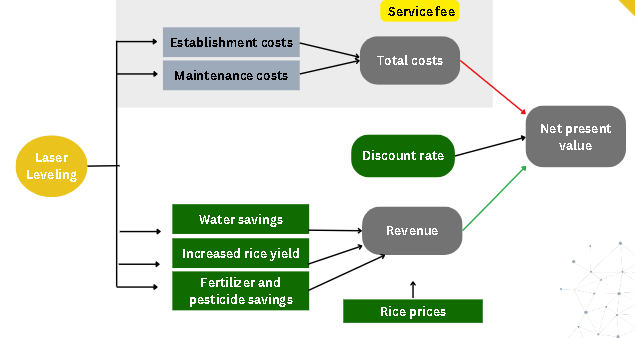
\includegraphics{images/conceptual_model-01.png}

\hypertarget{analysis}{%
\section{Analysis}\label{analysis}}

\hypertarget{cost-benefit-analysis}{%
\subsection{Cost-benefit Analysis}\label{cost-benefit-analysis}}

A cost-benefit analysis comparing the expenses associated with laser
leveling to the potential benefits it may bring to the farmer
cooperatives was conducted. The computations are done under the
assumptions below.

\hypertarget{assumption-sources-for-4w-tractor-laser-leveler}{%
\subsubsection{Assumption sources for 4W tractor laser
leveler:}\label{assumption-sources-for-4w-tractor-laser-leveler}}

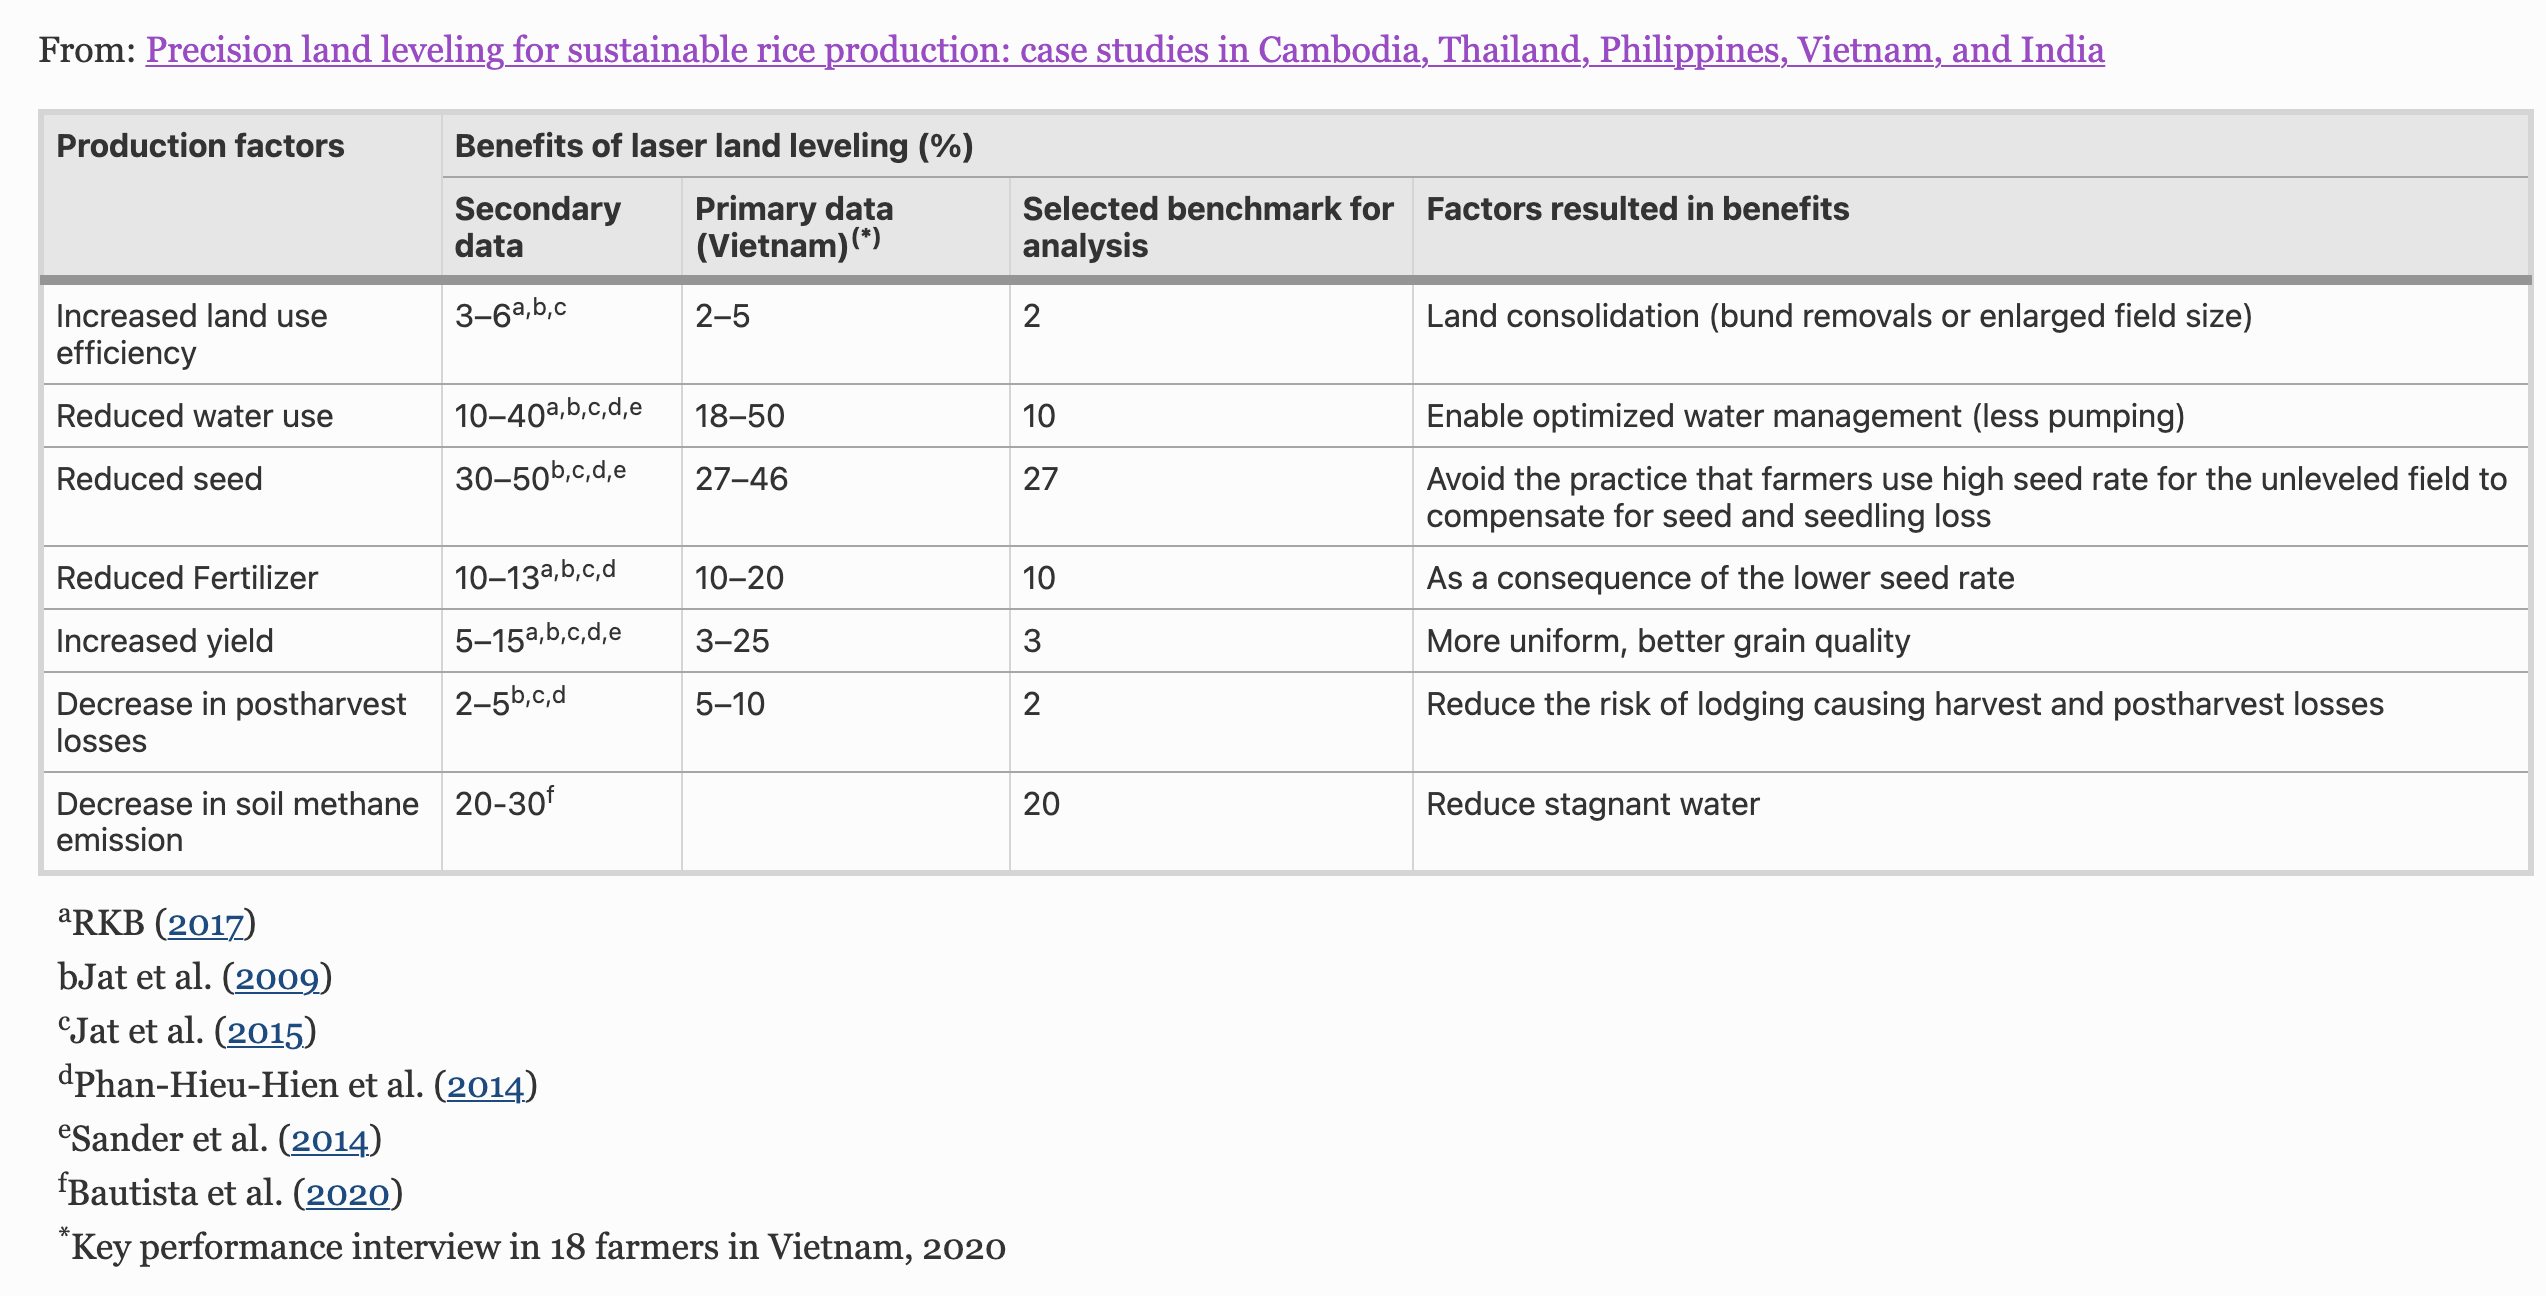
\includegraphics{images/Screenshot 2023-06-19 at 5.34.39 PM-01.png}

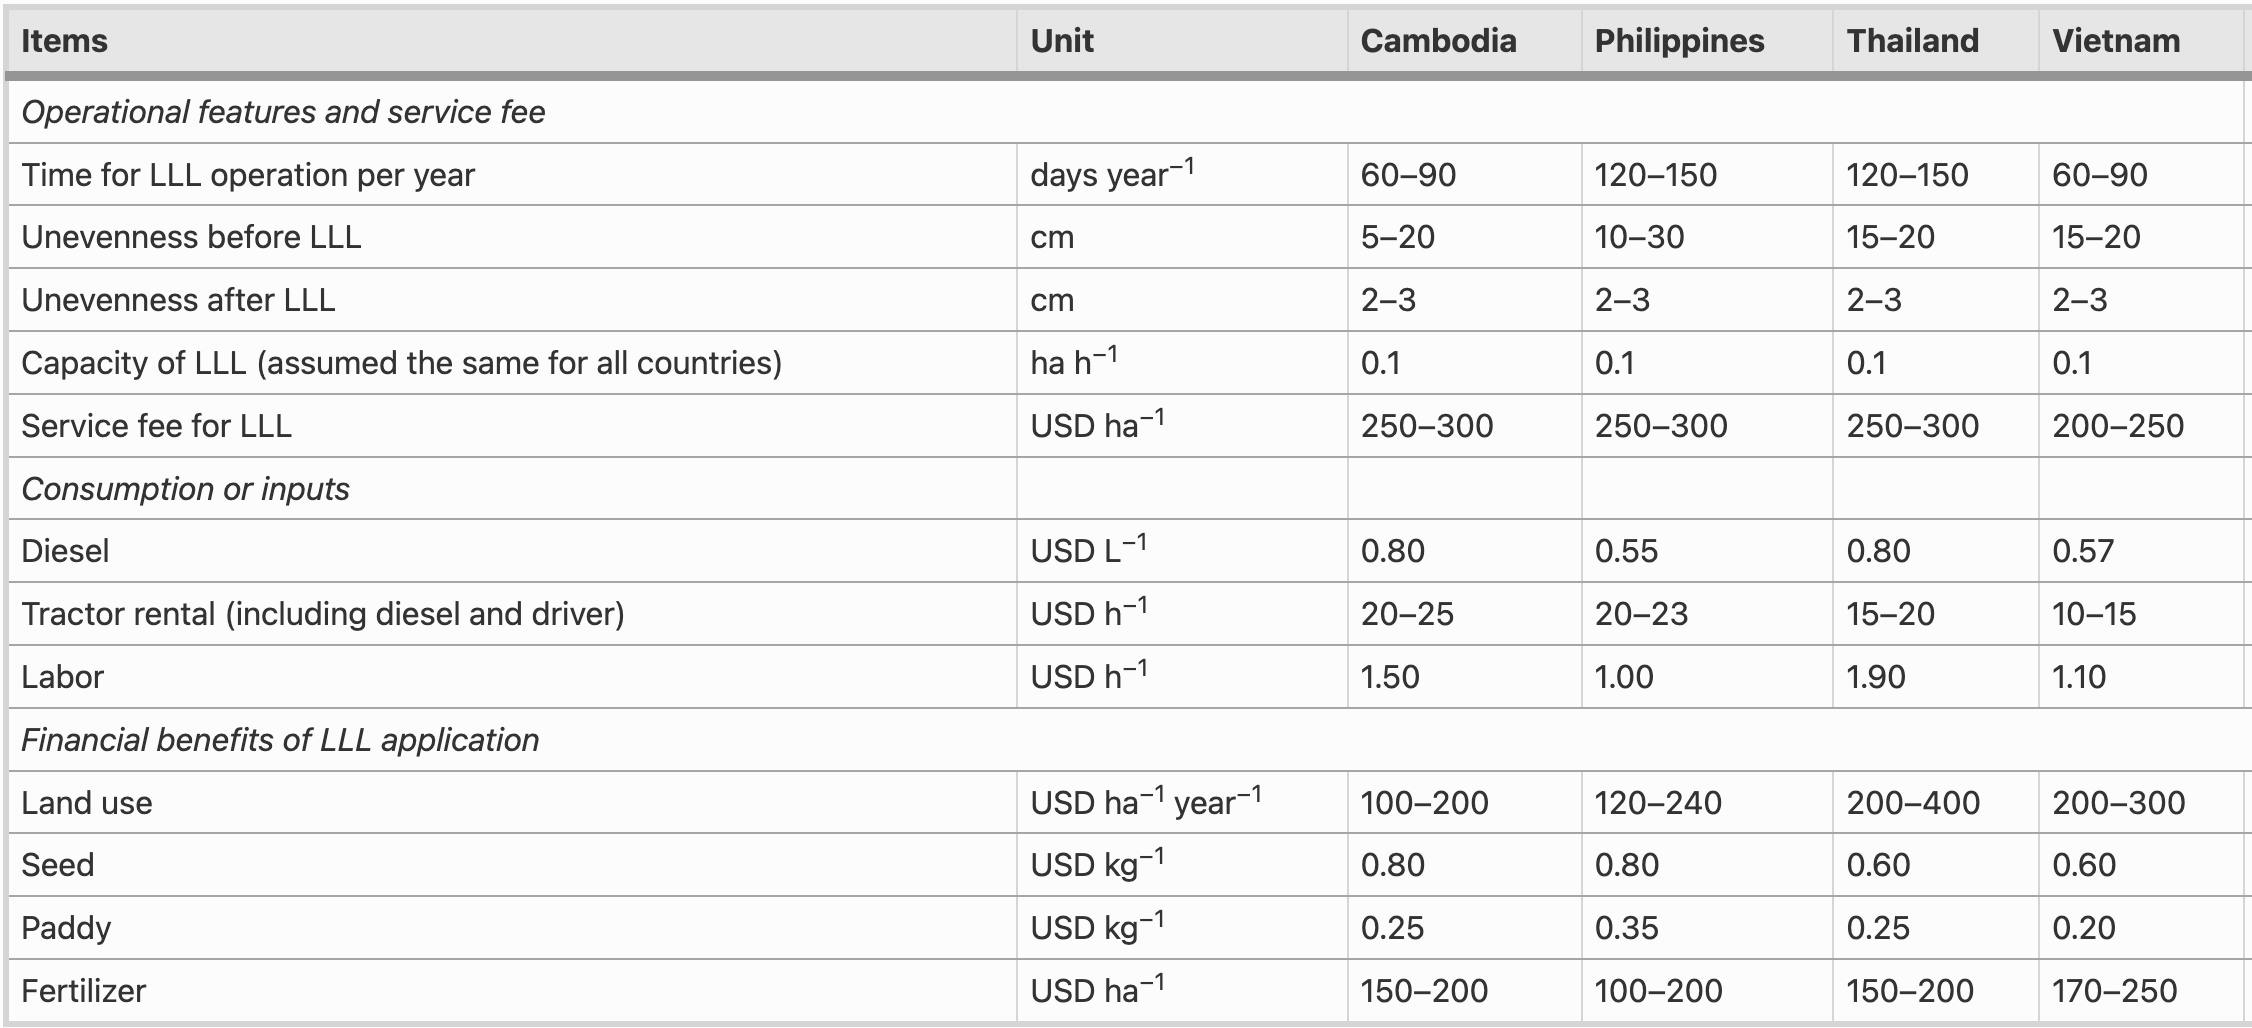
\includegraphics{images/Screenshot 2023-06-12 at 9.42.22 PM.png}

Source: (\textbf{nguyen-van-hung\_precision\_2022?})

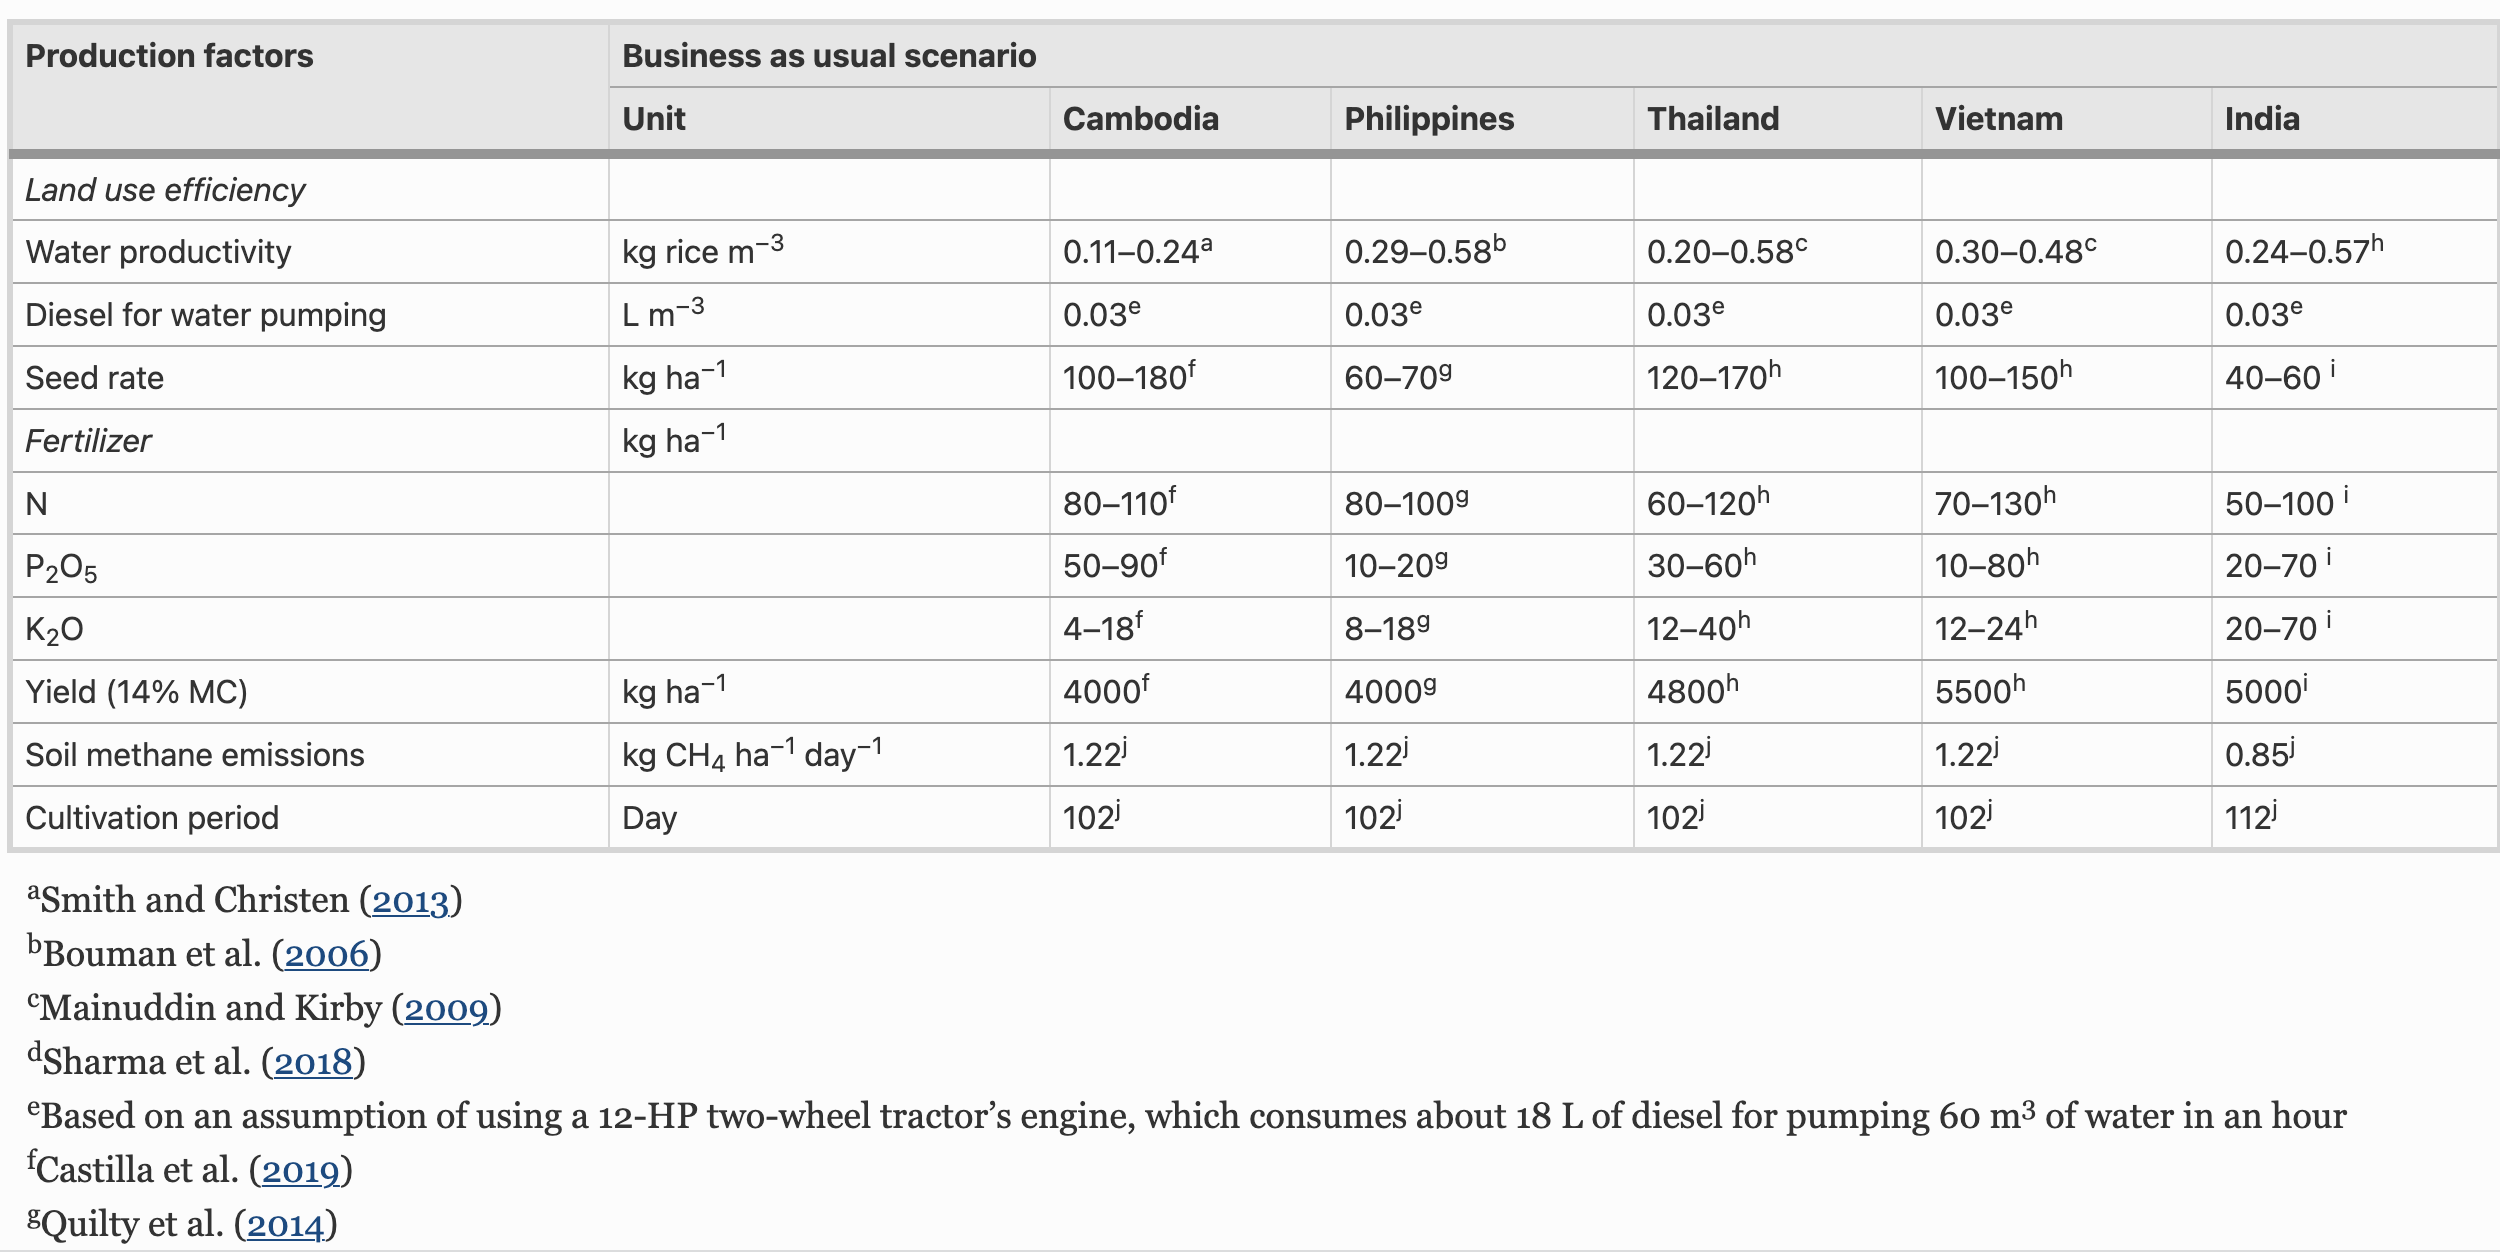
\includegraphics{images/Screenshot 2023-06-12 at 10.52.03 PM.png}

Source: (\textbf{nguyen-van-hung\_precision\_2022?})

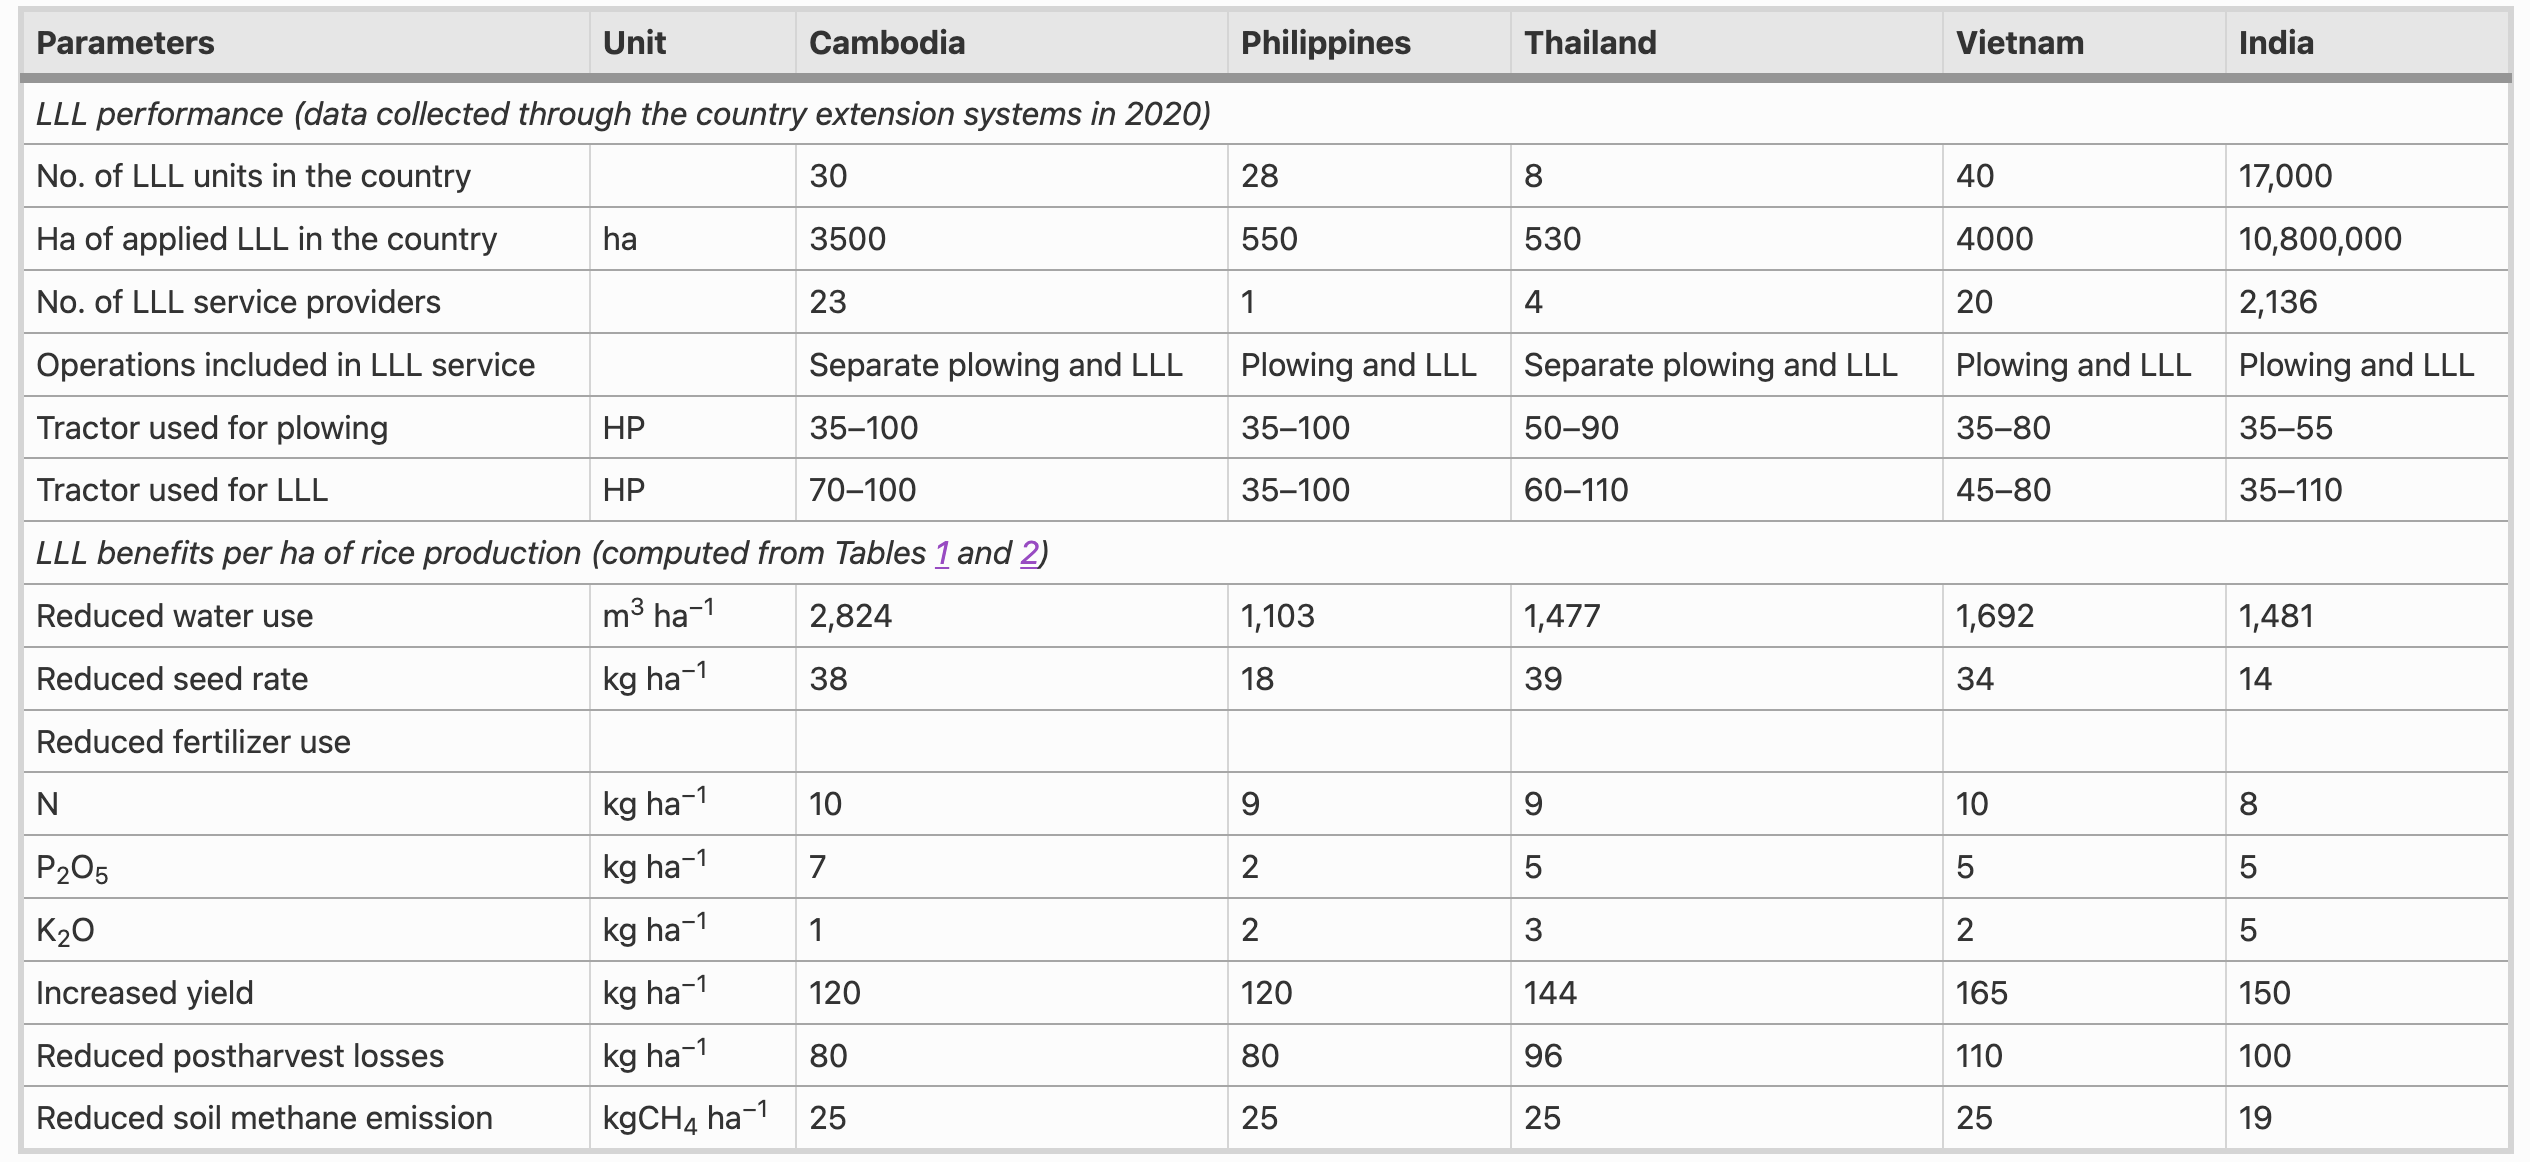
\includegraphics{images/Screenshot 2023-06-16 at 12.29.18 PM.png}

Source: (\textbf{nguyen-van-hung\_precision\_2022?})

20000 VND-\textgreater{} minimum wage in Region II Vietnam (Dat, 2023)

7.8\% interest rate -\textgreater{} current rate for short term loans in
Vietnam (Worldbank, 2021)

40-50 USD/hr-\textgreater{} service fee for plowing

10 cropping seasons-\textgreater LLL will be done every 5 years, and
rice production will be done every cropping season

20\% additional input cost per season for re-smoothing of field

\hypertarget{formulas-used}{%
\subsubsection{\texorpdfstring{\textbf{Formulas
used}}{Formulas used}}\label{formulas-used}}

𝐼𝑛𝐶𝑜𝑠𝑡𝑓𝑎𝑟𝑚𝑒𝑟=𝐹𝑒𝑒𝑠𝑒𝑟𝑣𝑖𝑐𝑒(1+0.2∗9)

𝑂𝑢𝑡𝑝𝑢𝑡𝑓𝑎𝑟𝑚𝑒𝑟=𝑃𝑟𝑜𝑓𝑖𝑡𝑠𝑒𝑎𝑠𝑜𝑛∗10

𝐼𝑛𝐶𝑜𝑠𝑡𝑠𝑒𝑟𝑣𝑖𝑐𝑒=𝐶𝑜𝑠𝑡𝐷𝑒𝑝𝑟𝑒𝑐𝑖𝑎𝑡𝑖𝑜𝑛+𝐼𝑛𝑡𝑒𝑟𝑒𝑠𝑡+𝐿𝑎𝑏𝑜𝑟+𝐹𝑢𝑒𝑙+𝑇𝑟𝑎𝑐𝑡𝑜𝑟𝑟𝑒𝑛𝑡𝑎𝑙+𝑀𝑎𝑛𝑎𝑔𝑒𝑚𝑒𝑛𝑡

𝑂𝑢𝑡𝑝𝑢𝑡𝑠𝑒𝑟𝑣𝑖𝑐𝑒=𝐹𝑒𝑒 𝑠𝑒𝑟𝑣𝑖𝑐𝑒

\hypertarget{code}{%
\subsubsection{Code}\label{code}}

\begin{Shaded}
\begin{Highlighting}[]
\FunctionTok{library}\NormalTok{(}\StringTok{"ggplot2"}\NormalTok{)}
\FunctionTok{library}\NormalTok{(dplyr)}
\CommentTok{\# cost analysis for LLL service provider (to be paid by farmer)}
\CommentTok{\#declaration of user input variables:}
\NormalTok{VND}\OtherTok{\textless{}{-}}\FloatTok{23487.50} \CommentTok{\#value of 1 USD to Vietnamese Dong (VND) as of date}
\DocumentationTok{\#\#\#operation (plowing, planting, harvest)}
\NormalTok{area\_covered}\OtherTok{\textless{}{-}} \DecValTok{3} \CommentTok{\#in ha}
\NormalTok{working\_days}\OtherTok{\textless{}{-}} \DecValTok{60} \CommentTok{\#in days}
\NormalTok{hours\_day}\OtherTok{\textless{}{-}}\DecValTok{8} \CommentTok{\#number of working hours per day}
\NormalTok{hrs\_area}\OtherTok{\textless{}{-}}\NormalTok{(area\_covered}\SpecialCharTok{/}\NormalTok{working\_days}\SpecialCharTok{/}\NormalTok{hours\_day)}\SpecialCharTok{*}\DecValTok{10000} \CommentTok{\#area to be covered in sq.m per hour}

\DocumentationTok{\#\#\#equipment sizing}
\NormalTok{speed\_op}\OtherTok{\textless{}{-}}\FloatTok{7.5} \CommentTok{\#speed of operation in km/hr}
\NormalTok{field\_ef}\OtherTok{\textless{}{-}}\DecValTok{40} \CommentTok{\#field efficiency in \%}
\NormalTok{LL\_size}\OtherTok{\textless{}{-}} \FloatTok{1.5} \CommentTok{\#commercially available size of drag bucket in m}
\NormalTok{actual\_area}\OtherTok{\textless{}{-}} \SpecialCharTok{+}\NormalTok{(LL\_size}\SpecialCharTok{*}\NormalTok{speed\_op)}\SpecialCharTok{*}\NormalTok{(field\_ef}\SpecialCharTok{/}\DecValTok{100}\NormalTok{)}\SpecialCharTok{*}\DecValTok{1000} \CommentTok{\#actual area covered in m2/hr}

\DocumentationTok{\#\#\#cost calculation}
\NormalTok{tractor\_price}\OtherTok{\textless{}{-}}\DecValTok{30000}\SpecialCharTok{*}\NormalTok{VND }\CommentTok{\#purchase price in Vietnamese Dong (VND)}
\NormalTok{usage\_tractor}\OtherTok{\textless{}{-}}\DecValTok{1200} \CommentTok{\#in hrs/yr}
\NormalTok{LL\_price}\OtherTok{\textless{}{-}}\DecValTok{12000}\SpecialCharTok{*}\NormalTok{VND }\CommentTok{\#purchase price of laser leveler in VND}
\NormalTok{usage\_LL}\OtherTok{\textless{}{-}} \SpecialCharTok{+}\NormalTok{working\_days}\SpecialCharTok{*}\NormalTok{hours\_day }\CommentTok{\#usage of laser leveler in hours/year}

\DocumentationTok{\#\#operating costs}
\NormalTok{engine\_power}\OtherTok{\textless{}{-}}\FloatTok{37.285} \CommentTok{\#in kW}

\NormalTok{fuel\_use}\OtherTok{\textless{}{-}}\SpecialCharTok{+}\NormalTok{engine\_power}\SpecialCharTok{/}\FloatTok{4.2} \CommentTok{\#in L}
\NormalTok{fuel\_cost}\OtherTok{\textless{}{-}}\FloatTok{22622.5} \CommentTok{\#in VND/L}
\NormalTok{fuel\_cost\_hr}\OtherTok{\textless{}{-}}\SpecialCharTok{+}\NormalTok{fuel\_cost}\SpecialCharTok{*}\NormalTok{fuel\_use }\CommentTok{\#fuel cost per hr}
\NormalTok{repair\_maintenance}\OtherTok{\textless{}{-}}\NormalTok{tractor\_price}\SpecialCharTok{/}\DecValTok{10}\SpecialCharTok{/}\NormalTok{usage\_tractor }\CommentTok{\#VND/hr}
\NormalTok{labor}\OtherTok{\textless{}{-}}\DecValTok{20000} \CommentTok{\#in VND/hr}
\NormalTok{total\_op\_cost}\OtherTok{\textless{}{-}}\SpecialCharTok{+}\NormalTok{repair\_maintenance}\SpecialCharTok{+}\NormalTok{fuel\_cost\_hr}\SpecialCharTok{+}\NormalTok{labor }\CommentTok{\#in VND/hr}

\DocumentationTok{\#\#fixed costs}
\NormalTok{tractor\_dep}\OtherTok{\textless{}{-}}\SpecialCharTok{+}\NormalTok{tractor\_price}\SpecialCharTok{/}\DecValTok{10}\SpecialCharTok{/}\NormalTok{usage\_tractor }\CommentTok{\#tractor depreciation in VND/hr}
\NormalTok{LL\_dep}\OtherTok{\textless{}{-}}\SpecialCharTok{+}\NormalTok{LL\_price}\SpecialCharTok{/}\DecValTok{10}\SpecialCharTok{/}\NormalTok{usage\_LL }\CommentTok{\#laser leveler depreciation in VND/hr}
\NormalTok{inv\_opp\_cost}\OtherTok{\textless{}{-}}\FloatTok{7.8} \CommentTok{\#investment/opportunity cost, a.k.a. interest for borrowing money}
\NormalTok{inv\_cost}\OtherTok{\textless{}{-}}\SpecialCharTok{+}\NormalTok{(tractor\_price}\SpecialCharTok{/}\NormalTok{usage\_tractor)}\SpecialCharTok{+}\NormalTok{((LL\_price}\SpecialCharTok{/}\NormalTok{usage\_LL)}\SpecialCharTok{*}\NormalTok{(inv\_opp\_cost}\SpecialCharTok{/}\DecValTok{100}\NormalTok{)) }\CommentTok{\#investment cost in VND/hr}
\NormalTok{total\_fixed\_cost}\OtherTok{\textless{}{-}}\NormalTok{tractor\_dep}\SpecialCharTok{+}\NormalTok{LL\_dep}\SpecialCharTok{+}\NormalTok{inv\_cost}

\NormalTok{total\_cost}\OtherTok{\textless{}{-}}\SpecialCharTok{+}\NormalTok{total\_op\_cost}\SpecialCharTok{+}\NormalTok{total\_fixed\_cost }\CommentTok{\#total cost in VND/hr}
\NormalTok{land\_lvl}\OtherTok{\textless{}{-}}\DecValTok{2} \CommentTok{\#average soil variation in cm}
\NormalTok{cost\_area}\OtherTok{\textless{}{-}}\NormalTok{total\_cost}\SpecialCharTok{/}\NormalTok{(actual\_area}\SpecialCharTok{/}\DecValTok{10000}\NormalTok{)}\SpecialCharTok{*}\NormalTok{land\_lvl }\CommentTok{\#cost/area in VND/ha}

\DocumentationTok{\#\#\#service provider}
\NormalTok{return\_mgt}\OtherTok{\textless{}{-}} \DecValTok{10} \CommentTok{\#return to management for operating the business in \%}
\NormalTok{service\_fee\_LLL}\OtherTok{\textless{}{-}}\NormalTok{(cost\_area}\SpecialCharTok{*}\NormalTok{((}\DecValTok{100}\SpecialCharTok{+}\NormalTok{return\_mgt)}\SpecialCharTok{/}\DecValTok{100}\NormalTok{))  }\CommentTok{\#in VND/ha, assuming LLL operation of 60 days per year}
\NormalTok{Input\_cost\_farmer}\OtherTok{\textless{}{-}}\NormalTok{service\_fee\_LLL}\SpecialCharTok{*}\NormalTok{(}\DecValTok{1}\FloatTok{+0.2}\SpecialCharTok{*}\DecValTok{9}\NormalTok{) }\CommentTok{\#in VND/ha under the assumption of LL operation every 5 years and resmoothing per season valued at 20\%}
\FunctionTok{print}\NormalTok{(Input\_cost\_farmer)}
\end{Highlighting}
\end{Shaded}

\begin{verbatim}
## [1] 14099185
\end{verbatim}

\begin{Shaded}
\begin{Highlighting}[]
\CommentTok{\#benefits for farmer}
\NormalTok{seed\_rate}\OtherTok{\textless{}{-}}\DecValTok{40} \CommentTok{\#kg/ha}
\NormalTok{yield}\OtherTok{\textless{}{-}}\DecValTok{5500} \CommentTok{\#at 14\% MC, kg/ha}
\NormalTok{N\_fert}\OtherTok{\textless{}{-}}\DecValTok{70} \CommentTok{\#kg/ha}
\NormalTok{P\_fert}\OtherTok{\textless{}{-}}\DecValTok{10} \CommentTok{\#kg/ha}
\NormalTok{K\_fert}\OtherTok{\textless{}{-}}\DecValTok{12} \CommentTok{\#kg/ha}
\NormalTok{land\_use}\OtherTok{\textless{}{-}}\DecValTok{200}\SpecialCharTok{*}\DecValTok{23487} \CommentTok{\#benefit in VND/ha/year}
\NormalTok{seed}\OtherTok{\textless{}{-}}\FloatTok{0.6}\SpecialCharTok{*}\DecValTok{23487} \CommentTok{\#benefit in VND/kg}
\NormalTok{paddy}\OtherTok{\textless{}{-}}\FloatTok{0.2}\SpecialCharTok{*}\DecValTok{23487} \CommentTok{\#benefit in VND/kg}
\NormalTok{fertilizer}\OtherTok{\textless{}{-}}\DecValTok{170}\SpecialCharTok{*}\DecValTok{23487} \CommentTok{\#benefit in VND/ha}
\NormalTok{season\_profit}\OtherTok{\textless{}{-}}\NormalTok{ ((land\_use)}\SpecialCharTok{/}\DecValTok{2}\NormalTok{)}\SpecialCharTok{+}\NormalTok{(seed}\SpecialCharTok{*}\NormalTok{seed\_rate)}\SpecialCharTok{+}\NormalTok{ (paddy}\SpecialCharTok{*}\NormalTok{seed\_rate) }\SpecialCharTok{+}\NormalTok{ (fertilizer)}\CommentTok{\#profit from season\textquotesingle{}s yields and savings after LLL in VND/ha}
\NormalTok{Output\_farmer}\OtherTok{\textless{}{-}}\NormalTok{ season\_profit }\SpecialCharTok{*}\DecValTok{10} \CommentTok{\#VND/ha for 10 cropping seasons}
\FunctionTok{print}\NormalTok{(Output\_farmer)}
\end{Highlighting}
\end{Shaded}

\begin{verbatim}
## [1] 70930740
\end{verbatim}

\begin{Shaded}
\begin{Highlighting}[]
\CommentTok{\#benefit{-}cost ratio}
\NormalTok{BC\_ratio}\OtherTok{\textless{}{-}}\NormalTok{ Output\_farmer}\SpecialCharTok{/}\NormalTok{Input\_cost\_farmer}
\FunctionTok{print}\NormalTok{(BC\_ratio)}
\end{Highlighting}
\end{Shaded}

\begin{verbatim}
## [1] 5.03084
\end{verbatim}

\begin{Shaded}
\begin{Highlighting}[]
\CommentTok{\#data visualization}
\NormalTok{cost\_shares}\OtherTok{\textless{}{-}}\FunctionTok{data.frame}\NormalTok{(}\AttributeTok{Portions=}\FunctionTok{c}\NormalTok{(}\StringTok{"Fuel consumption"}\NormalTok{,}\StringTok{"Repair and maintenance"}\NormalTok{,}\StringTok{"Labor cost"}\NormalTok{, }\StringTok{"Tractor depreciation"}\NormalTok{,}\StringTok{"Laser leveler depreciation"}\NormalTok{, }\StringTok{"Investment cost"}\NormalTok{), }\AttributeTok{share=}\FunctionTok{c}\NormalTok{(fuel\_cost\_hr, repair\_maintenance, labor, tractor\_dep, LL\_dep, inv\_cost))}


\NormalTok{cost\_shares }\OtherTok{\textless{}{-}}\NormalTok{ cost\_shares }\SpecialCharTok{\%\textgreater{}\%}
  \FunctionTok{arrange}\NormalTok{(}\FunctionTok{desc}\NormalTok{(Portions)) }\SpecialCharTok{\%\textgreater{}\%}
  \FunctionTok{mutate}\NormalTok{(}\AttributeTok{lab.ypos =} \FunctionTok{cumsum}\NormalTok{(share) }\SpecialCharTok{{-}} \FloatTok{0.5}\SpecialCharTok{*}\NormalTok{share)}

\NormalTok{mycols }\OtherTok{\textless{}{-}} \FunctionTok{c}\NormalTok{(}\StringTok{"\#0073C2FF"}\NormalTok{, }\StringTok{"\#EFC000FF"}\NormalTok{, }\StringTok{"\#868686FF"}\NormalTok{, }\StringTok{"\#CD534CFF"}\NormalTok{, }\StringTok{"\#00BA38"}\NormalTok{,}\StringTok{"\#A020F0"}\NormalTok{)}

\FunctionTok{ggplot}\NormalTok{(cost\_shares, }\FunctionTok{aes}\NormalTok{(}\AttributeTok{x =} \StringTok{""}\NormalTok{, }\AttributeTok{y =}\NormalTok{ share, }\AttributeTok{fill =}\NormalTok{ Portions)) }\SpecialCharTok{+}
  \FunctionTok{geom\_bar}\NormalTok{(}\AttributeTok{width =} \DecValTok{1}\NormalTok{, }\AttributeTok{stat =} \StringTok{"identity"}\NormalTok{, }\AttributeTok{color =} \StringTok{"white"}\NormalTok{) }\SpecialCharTok{+}
  \FunctionTok{coord\_polar}\NormalTok{(}\StringTok{"y"}\NormalTok{, }\AttributeTok{start =} \DecValTok{0}\NormalTok{)}\SpecialCharTok{+}
  \FunctionTok{geom\_text}\NormalTok{(}\FunctionTok{aes}\NormalTok{(}\AttributeTok{y =}\NormalTok{ lab.ypos, }\AttributeTok{label =}\StringTok{" "}\NormalTok{), }\AttributeTok{color =} \StringTok{"white"}\NormalTok{)}\SpecialCharTok{+}
  \FunctionTok{scale\_fill\_manual}\NormalTok{(}\AttributeTok{values =}\NormalTok{ mycols) }\SpecialCharTok{+}
  \FunctionTok{theme\_void}\NormalTok{()}
\end{Highlighting}
\end{Shaded}

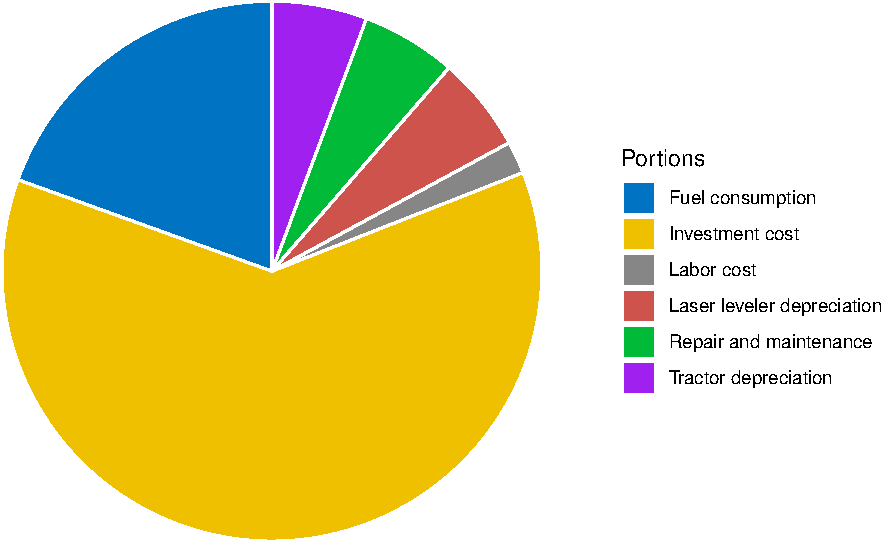
\includegraphics{Laser_leveling_simulation_files/figure-latex/cost-benefit-analysis-1.pdf}

Figure X. Cost proportions of LLL.

\begin{Shaded}
\begin{Highlighting}[]
\CommentTok{\# data loading and sorting R code:}
\NormalTok{cost\_area}
\end{Highlighting}
\end{Shaded}

\begin{verbatim}
## [1] 4577657
\end{verbatim}

\hypertarget{yield-analysis}{%
\subsection{Yield Analysis}\label{yield-analysis}}

Performing an analysis to determine the potential yield improvement
laser leveling could offer in comparison to tradtional farming.

\hypertarget{assumption-sources}{%
\subsubsection{Assumption sources:}\label{assumption-sources}}

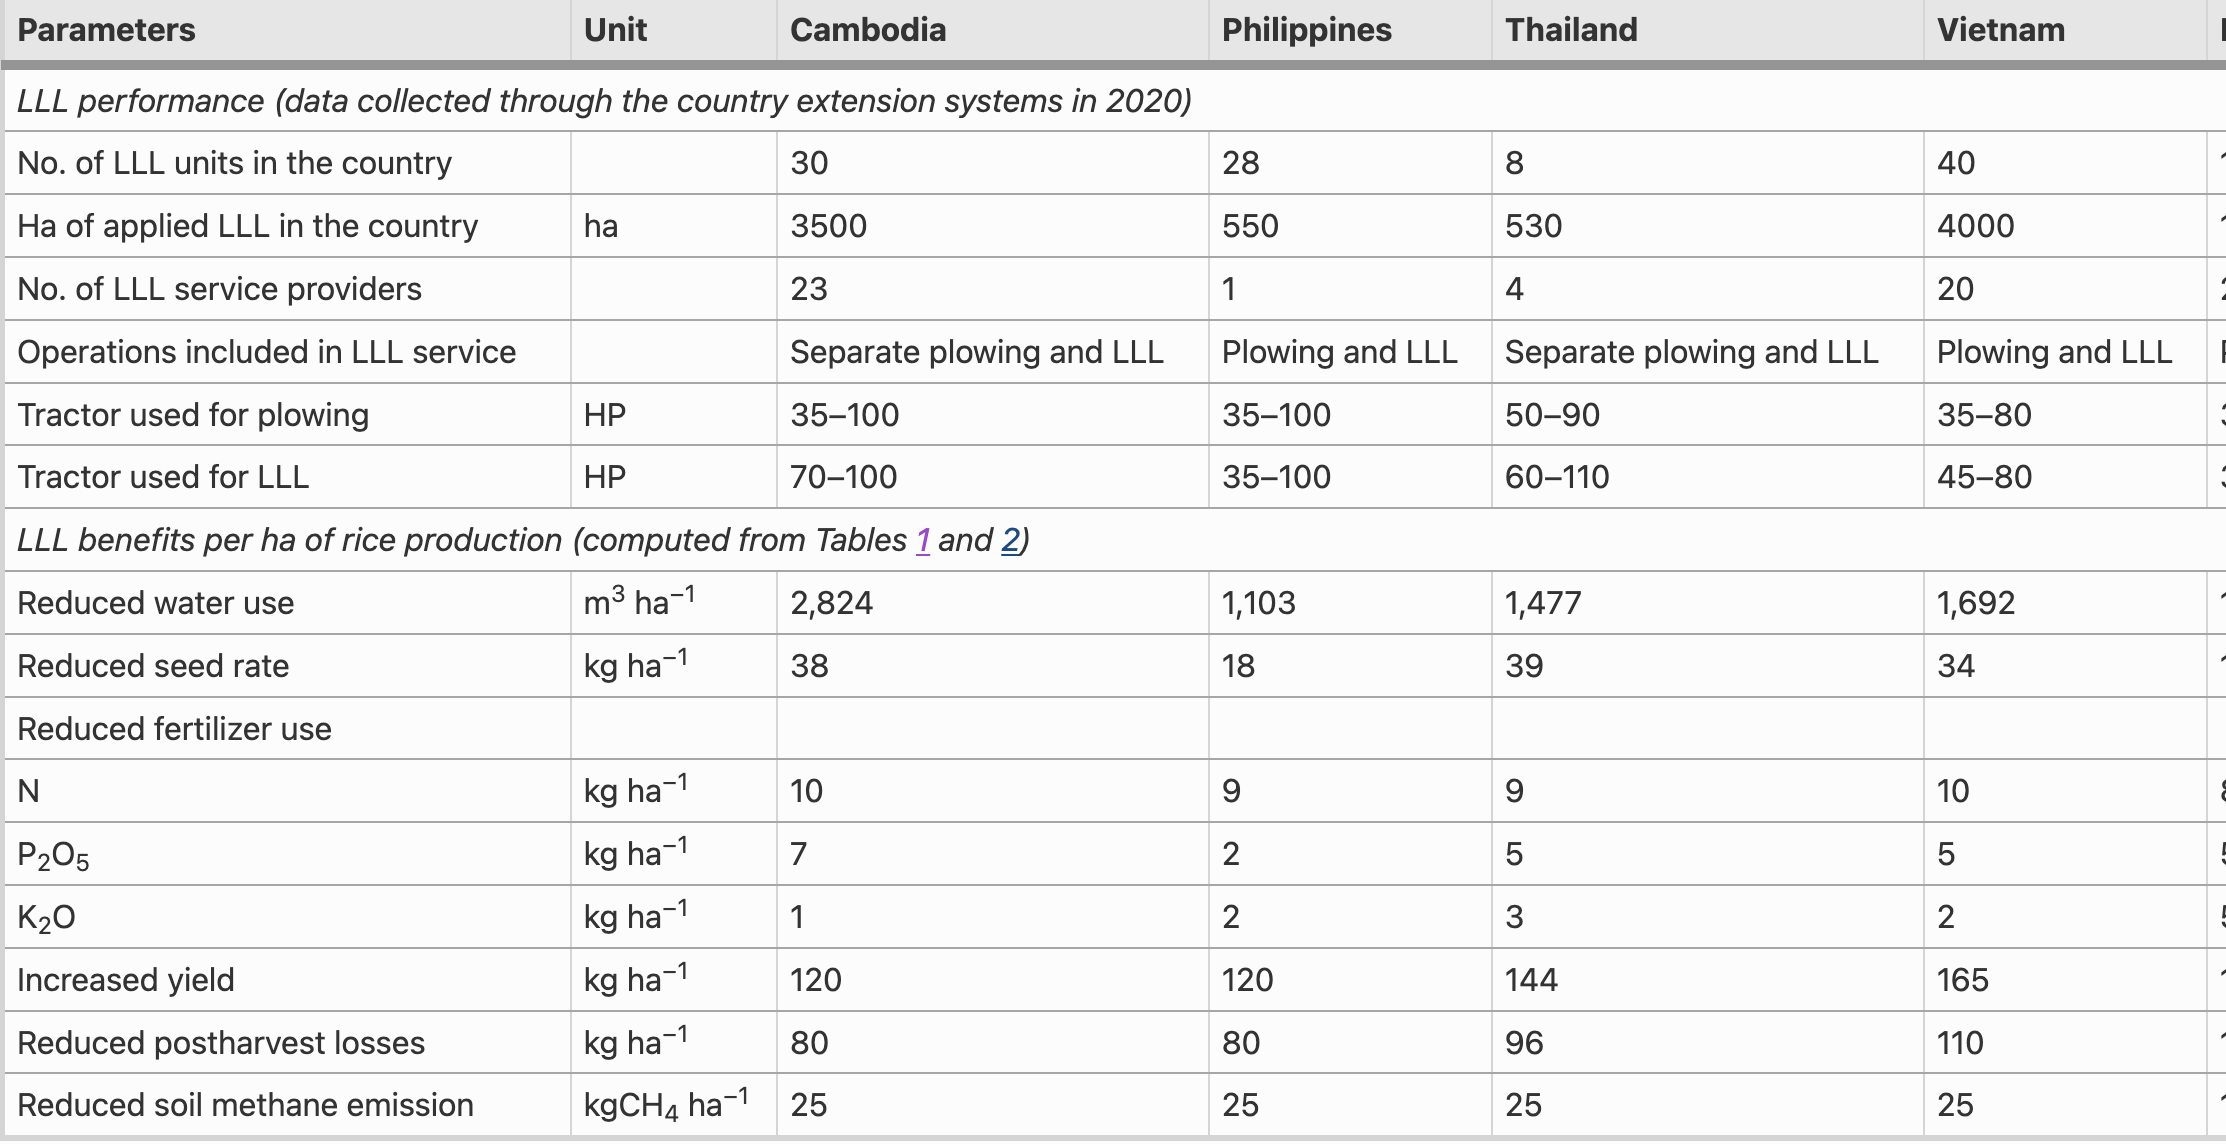
\includegraphics{images/Screenshot 2023-06-12 at 9.38.09 PM.png}

Source: (\textbf{nguyen-van-hung\_precision\_2022?})

\begin{Shaded}
\begin{Highlighting}[]
\CommentTok{\# yield analysis R:}

\NormalTok{yield\_weight}\OtherTok{\textless{}{-}} \DecValTok{0} \CommentTok{\#weight of yield (total grains harvested in field at 14\% MC) in kg}
\NormalTok{field\_size}\OtherTok{\textless{}{-}}\DecValTok{0}  \CommentTok{\#typical field size in Vietnam in ha}
\NormalTok{GY}\OtherTok{\textless{}{-}}\NormalTok{ yield\_weight}\SpecialCharTok{/}\NormalTok{field\_size}
\end{Highlighting}
\end{Shaded}

\hypertarget{sensitivity-analysis}{%
\subsection{Sensitivity Analysis}\label{sensitivity-analysis}}

Conducting a sensitivity analysis to assess the impact of varying key
parameters and assumptions on the decision outcome. Maybe explore
different scenarios and evaluate their influence on the decision to
adopt laser leveling?

\begin{Shaded}
\begin{Highlighting}[]
\CommentTok{\# sensitivity analysis R code:}
\end{Highlighting}
\end{Shaded}

\hypertarget{results}{%
\section{Results}\label{results}}

\hypertarget{monte-carlo-simulation-for-business-as-usual-scenario}{%
\subsection{Monte Carlo Simulation for business as usual
scenario}\label{monte-carlo-simulation-for-business-as-usual-scenario}}

``\,``\,'' investment\_LL = TRUE n\_years = 25 establishment\_cost\_LL =
cost\_area \# assuming 1 hectar right now maintenance\_cost =
(establishment\_cost\_LLL * 0.8)/5 \# fictive assumtion that maintenance
costs are 80\% of initial investment costs each 5 years Yield = 5400 \#
assuming 5.4 tons for testing Market\_price = 0.439 * VND \# 0.439 USD
times VND exchange rate intervention\_communication\_cost = 200 * VND
intervention\_zoning\_cost = 150 * VND \# Estimate the income in a
normal season income\_norm \textless- Yield * Market\_price ``\,``\,''

\begin{Shaded}
\begin{Highlighting}[]
\NormalTok{LL\_model\_function }\OtherTok{\textless{}{-}} \ControlFlowTok{function}\NormalTok{(x, varnames)\{}
  
    \CommentTok{\# calculate ex{-}ante risks: impact the implementation of interventions \#\#\#\#}
  \CommentTok{\#}
\NormalTok{    intervention\_No\_coop\_Event }\OtherTok{\textless{}{-}} \FunctionTok{chance\_event}\NormalTok{(chance\_noLL, }\DecValTok{1}\NormalTok{, }\DecValTok{0}\NormalTok{, }\AttributeTok{n =} \DecValTok{1}\NormalTok{)}
  \CommentTok{\# chance\_event chooses with probability "intervention\_NonColabInvolv" the first scenario (1 in this case), otherwise 0 (no involvement)}
  
  \CommentTok{\#precalculation of common random draws for all intervention model runs}
  \CommentTok{\# benefits of rice cultivation WITH LLL:        }
    
\DocumentationTok{\#\#\#\#\#\#ARE WE GOING TO LEAVE THIS ABOUT THE INPUT VALUES? SHOULDNT WE DELETE IT??}\AlertTok{\#\#\#}

            \CommentTok{\# \#\#reference for the units used in precalculations, these are values per season, and there are 2 seasons per year:}
            \CommentTok{\# seed\_rate\textless{}{-}40 \#kg/ha}
            \CommentTok{\# yield\textless{}{-}5500 \#at 14\% MC, kg/ha}
            \CommentTok{\# N\_fert\textless{}{-}70 \#kg/ha}
            \CommentTok{\# P\_fert\textless{}{-}10 \#kg/ha}
            \CommentTok{\# K\_fert\textless{}{-}12 \#kg/ha}
            \CommentTok{\# land\_use\textless{}{-}200*23487 \#benefit in VND/ha/year}
            \CommentTok{\# seed\textless{}{-}0.6*23487 \#benefit in VND/kg}
            \CommentTok{\# paddy\textless{}{-}0.2*23487 \#benefit in VND/kg}
            \CommentTok{\# fertilizer\textless{}{-}170*23487 \#benefit in VND/ha}
            \CommentTok{\# season\_profit\textless{}{-} ((land\_use)/2)+(seed*seed\_rate)+ (paddy*seed\_rate) + (fertilizer)\#profit from season\textquotesingle{}s yields and savings after LLL in VND/ha}
            \CommentTok{\# Output\_farmer\textless{}{-} season\_profit *10 \#VND/ha for 10 cropping seasons                                      }
  \CommentTok{\# Precalculationn for the change in yield with the intervention of Laser Leveling}
\NormalTok{  precalc\_LL\_yield }\OtherTok{\textless{}{-}}
    \FunctionTok{vv}\NormalTok{(yield\_LL, var\_CV, n\_years) }\SpecialCharTok{*} \CommentTok{\# yield [t/ha]}
    \FunctionTok{vv}\NormalTok{(farm\_area, var\_CV, n\_years) }\SpecialCharTok{*} \CommentTok{\# area of the field per farmer [ha]}
    \FunctionTok{vv}\NormalTok{(rice\_price, var\_CV, n\_years) }\CommentTok{\# rice price [USD/t]}
  
  \CommentTok{\# Precalculationn for the water savings with the intervention of Laser Leveling}
\NormalTok{  precalc\_LL\_water\_savings }\OtherTok{\textless{}{-}}
    \FunctionTok{vv}\NormalTok{(LL\_water\_saving, var\_CV, n\_years) }\SpecialCharTok{*} \CommentTok{\# water savings in [m\^{}3/ha]}
    \FunctionTok{vv}\NormalTok{(LL\_water\_cost, var\_CV, n\_years) }\CommentTok{\# cost of irrigation water [USD/m\^{}3]}
  
  \CommentTok{\# Precalculationn for the fertilizer savings with the intervention of Laser Leveling}
\NormalTok{  precalc\_LL\_fert\_savings }\OtherTok{\textless{}{-}}
\NormalTok{    (}\FunctionTok{vv}\NormalTok{(Fertilizer\_cost\_noLL, var\_CV, n\_years) }\SpecialCharTok{{-}} \CommentTok{\# fertilizer cost w/o LL [USD/ha]}
    \FunctionTok{vv}\NormalTok{(Fertilizer\_cost\_LL, var\_CV, n\_years)) }\SpecialCharTok{*} \CommentTok{\# fertilizer cost with LL [USD/ha]}
    \FunctionTok{vv}\NormalTok{(farm\_area, var\_CV, n\_years) }\CommentTok{\# area of the field per farmer [ha]}
  
  \CommentTok{\# Precalculationn for the pesticide savings with the intervention of Laser Leveling}
\NormalTok{  precalc\_LL\_pest\_savings }\OtherTok{\textless{}{-}}
\NormalTok{    (}\FunctionTok{vv}\NormalTok{(Pesticide\_cost\_noLL, var\_CV, n\_years) }\SpecialCharTok{{-}} \CommentTok{\# pesticide cost w/o LL [USD/ha]}
    \FunctionTok{vv}\NormalTok{(Pesticide\_cost\_LL, var\_CV, n\_years)) }\SpecialCharTok{*} \CommentTok{\# pesticide cost with LL [USD/ha]}
    \FunctionTok{vv}\NormalTok{(farm\_area, var\_CV, n\_years) }\CommentTok{\# area of the field per farmer [ha]}
  
  \CommentTok{\# Precalculationn for the seed savings with the intervention of Laser Leveling}
\NormalTok{  precalc\_LL\_seed\_savings }\OtherTok{\textless{}{-}}
\NormalTok{    (}\FunctionTok{vv}\NormalTok{(Seed\_cost\_noLL, var\_CV, n\_years) }\SpecialCharTok{{-}} \CommentTok{\# seed cost w/o LL [USD/ha]}
    \FunctionTok{vv}\NormalTok{(Seed\_cost\_LL , var\_CV, n\_years)) }\SpecialCharTok{*} \CommentTok{\# seed cost with LL [USD/ha]}
    \FunctionTok{vv}\NormalTok{(farm\_area, var\_CV, n\_years) }\CommentTok{\# area of the field per farmer [ha]}
  
  \CommentTok{\# Precalculationn for the fuel savings with the intervention of Laser Leveling}
\NormalTok{  precalc\_LL\_fuel\_savings }\OtherTok{\textless{}{-}}
\NormalTok{    (}\FunctionTok{vv}\NormalTok{(Water\_pumping\_fuel\_cost\_noLL, var\_CV, n\_years) }\SpecialCharTok{{-}} \CommentTok{\# fuel w/o LL [USD/ha]}
    \FunctionTok{vv}\NormalTok{(Water\_pumping\_fuel\_cost\_LL, var\_CV, n\_years)) }\SpecialCharTok{*} \CommentTok{\# fuel cost with LL [USD/ha]}
    \FunctionTok{vv}\NormalTok{(farm\_area, var\_CV, n\_years) }\CommentTok{\# area of the field per farmer [ha]}
  
  \CommentTok{\# Precalculationn for the labor cost savings with the intervention of Laser Leveling}
\NormalTok{  precalc\_LL\_labor\_savings }\OtherTok{\textless{}{-}}
\NormalTok{    (}\FunctionTok{vv}\NormalTok{(Labor\_cost\_noLL, var\_CV, n\_years) }\SpecialCharTok{{-}} \CommentTok{\# labor w/o LL [USD/ha]}
    \FunctionTok{vv}\NormalTok{(Labor\_cost\_LL , var\_CV, n\_years)) }\SpecialCharTok{*} \CommentTok{\# labor cost with LL [USD/ha]}
    \FunctionTok{vv}\NormalTok{(farm\_area, var\_CV, n\_years) }\CommentTok{\# area of the field per farmer [ha]}
  
  \CommentTok{\# ASK GRACE {-}please explain}
  \CommentTok{\# Precalculationn for the change in land use with the intervention of Laser Leveling}
\NormalTok{   precalc\_LL\_land\_use }\OtherTok{\textless{}{-}}
    \FunctionTok{vv}\NormalTok{(LL\_land\_USD\_ha\_year, var\_CV, n\_years) }\SpecialCharTok{*}
    \FunctionTok{vv}\NormalTok{(farm\_area, var\_CV, n\_years) }
  
  
\NormalTok{  precalc\_LL }\OtherTok{\textless{}{-}}
\NormalTok{    precalc\_LL\_yield }\SpecialCharTok{+} 
\NormalTok{    precalc\_LL\_water\_savings }\SpecialCharTok{+}
\NormalTok{    precalc\_LL\_fert\_savings }\SpecialCharTok{+} 
\NormalTok{    precalc\_LL\_pest\_savings }\SpecialCharTok{+} 
\NormalTok{    precalc\_LL\_seed\_savings }\SpecialCharTok{+}
\NormalTok{    precalc\_LL\_labor\_savings }\SpecialCharTok{+}
\NormalTok{    precalc\_LL\_fuel\_savings }\SpecialCharTok{+} 
\NormalTok{    precalc\_LL\_land\_use}
    
    
    \CommentTok{\# benefits of rice cultivation WITHOUT LL:}
\NormalTok{  precalc\_conv\_prod }\OtherTok{\textless{}{-}}
    \FunctionTok{vv}\NormalTok{(yield\_noLL, var\_CV, n\_years) }\SpecialCharTok{*} \CommentTok{\# yield [t/ha]}
    \FunctionTok{vv}\NormalTok{(farm\_area, var\_CV, n\_years) }\SpecialCharTok{*} \CommentTok{\# area of the field per farmer [ha]}
    \FunctionTok{vv}\NormalTok{(rice\_price, var\_CV, n\_years) }\CommentTok{\# rice price [USD/t]}
  
  
  \DocumentationTok{\#\#\#\#  Intervention Preamble \#\#\#\#}
  
  \CommentTok{\# Run a simulation for both the application of LL and the conventional scenario without it:}
  \ControlFlowTok{for}\NormalTok{ (intervention\_LL }\ControlFlowTok{in} \FunctionTok{c}\NormalTok{(}\ConstantTok{FALSE}\NormalTok{,}\ConstantTok{TRUE}\NormalTok{))}
\NormalTok{      \{}
  
  \CommentTok{\# Set the preambles for the case if LLL application:    }
  \ControlFlowTok{if}\NormalTok{ (intervention\_LL)}
\NormalTok{  \{}
\NormalTok{    event\_LL }\OtherTok{\textless{}{-}} \ConstantTok{TRUE}
\NormalTok{    event\_LL\_cost }\OtherTok{\textless{}{-}} \ConstantTok{TRUE}
\NormalTok{    event\_LL\_PlanningCost }\OtherTok{\textless{}{-}} \ConstantTok{TRUE}
\NormalTok{    event\_conv\_rice\_prod }\OtherTok{\textless{}{-}} \ConstantTok{FALSE}
  \CommentTok{\# Set the preambles for the normal rice production scenario}
\NormalTok{  \} }\ControlFlowTok{else}
\NormalTok{  \{}
\NormalTok{    event\_LL }\OtherTok{\textless{}{-}} \ConstantTok{FALSE}
\NormalTok{    event\_LL\_cost }\OtherTok{\textless{}{-}} \ConstantTok{FALSE}
\NormalTok{    event\_LL\_PlanningCost }\OtherTok{\textless{}{-}} \ConstantTok{FALSE}
\NormalTok{    event\_conv\_rice\_prod }\OtherTok{\textless{}{-}} \ConstantTok{TRUE}
\NormalTok{  \}}
  
  \ControlFlowTok{if}\NormalTok{ (intervention\_No\_coop\_Event) \{}
    \CommentTok{\# only relevant if selected by chance and = TRUE}
    \CommentTok{\# if this condition is TRUE the implementation of LLL will be planned but not executed}
\NormalTok{    event\_LL }\OtherTok{\textless{}{-}} \ConstantTok{FALSE} \CommentTok{\# no LLL applied}
\NormalTok{    event\_LL\_cost }\OtherTok{\textless{}{-}} \ConstantTok{FALSE} \CommentTok{\# no establishment costs are created (planning costs however may occur)}
\NormalTok{    event\_LL\_PlanningCost }\OtherTok{\textless{}{-}} \ConstantTok{TRUE}
\NormalTok{    event\_conv\_rice\_prod }\OtherTok{\textless{}{-}} \ConstantTok{TRUE} \CommentTok{\# the normal scenario takes place}
\NormalTok{\}}
    
  \DocumentationTok{\#\#\#\#  Intervention \#\#\#\#}
  
  \CommentTok{\# summing up the investment costs if LLL is applied or not}
  \ControlFlowTok{if}\NormalTok{ (event\_LL\_cost) \{}
\NormalTok{    investment\_cost\_LL }\OtherTok{\textless{}{-}}\NormalTok{ establishment\_cost\_LL}
\NormalTok{  \} }\ControlFlowTok{else}
\NormalTok{    investment\_cost\_LL }\OtherTok{\textless{}{-}} \DecValTok{0}
  
  \CommentTok{\# calculating the planning costs \#\#\#\#\#\#\#\#MAYBE DONT USE\#\#\#\#\#\#\#\#}
  \ControlFlowTok{if}\NormalTok{ (event\_LL\_PlanningCost) \{}
\NormalTok{    plan\_cost\_intervention\_LL }\OtherTok{\textless{}{-}}\NormalTok{ planning\_cost\_LL }\SpecialCharTok{+} 
\NormalTok{                                  zoning\_cost\_LL}
\NormalTok{  \} }\ControlFlowTok{else}
\NormalTok{    plan\_cost\_intervention\_LL }\OtherTok{\textless{}{-}} \DecValTok{0}
  
  \CommentTok{\# calculating the maintenance costs, initializing the array with 0 costs for the first year:}
\NormalTok{  maintenance\_cost }\OtherTok{\textless{}{-}} \FunctionTok{rep}\NormalTok{(}\DecValTok{0}\NormalTok{, n\_years) }
  
  \CommentTok{\# Cost of the application of LLL per year }
  \ControlFlowTok{if}\NormalTok{ (event\_LL\_cost)}
\NormalTok{    maintenance\_cost }\OtherTok{\textless{}{-}}
\NormalTok{    maintenance\_cost }\SpecialCharTok{+} 
    \CommentTok{\# add a variation of the variable over the years}
\NormalTok{    decisionSupport}\SpecialCharTok{::}\FunctionTok{vv}\NormalTok{(maintenance\_cost\_LL, var\_CV, n\_years)}
  
  \CommentTok{\# First, all maintenance costs are stored in the variable:}
\NormalTok{  intervention\_cost }\OtherTok{\textless{}{-}}\NormalTok{ maintenance\_cost}
  
    \CommentTok{\# in the first year the establishment costs and planning costs are added:}
\NormalTok{  intervention\_cost[}\DecValTok{1}\NormalTok{] }\OtherTok{\textless{}{-}}
\NormalTok{    intervention\_cost[}\DecValTok{1}\NormalTok{] }\SpecialCharTok{+}  \CommentTok{\# equal to maintenance\_cost [1]}
\NormalTok{    investment\_cost\_LL }\SpecialCharTok{+}    \CommentTok{\# equal to establishment costs}
\NormalTok{    plan\_cost\_intervention\_LL}
  
  
   \DocumentationTok{\#\#\#\# Benefits from  cultivation in the intervention strips \#\#\#\#}
  
  \CommentTok{\# Now all benefits of the intervention will be calculated}
  \CommentTok{\# event\_LL is 0 if the introduction of LL does not take place, thereby the gains would be multiplied by 0 = become 0}
  
  \CommentTok{\# Benefits of intervention LLL:}
\NormalTok{  intervention\_LL\_benefits }\OtherTok{\textless{}{-}}
    \FunctionTok{as.numeric}\NormalTok{(event\_LL) }\SpecialCharTok{*}\NormalTok{ precalc\_LL}
  
  \CommentTok{\# Benefits of conventional rice production (ground truth):}
\NormalTok{  no\_LL\_benefits }\OtherTok{\textless{}{-}}
    \FunctionTok{as.numeric}\NormalTok{(event\_conv\_rice\_prod) }\SpecialCharTok{*}\NormalTok{   precalc\_conv\_prod}

  
  
  \DocumentationTok{\#\#\#\# Total benefits from rice production \#\#\#\#}
  
  \CommentTok{\# combined benefits (in reality: intervention\_LL\_benefits + 0 OR no\_LL\_benefits + 0)}
  \CommentTok{\#rice\_production \textless{}{-} intervention\_LL\_benefits + no\_LL\_benefits \#not needed since we separate the cases in the next part}
  
  
  \CommentTok{\# if the decision was to implement LL:}
  \ControlFlowTok{if}\NormalTok{ (intervention\_LL)\{}
\NormalTok{    net\_benefits }\OtherTok{\textless{}{-}}\NormalTok{ intervention\_LL\_benefits }\SpecialCharTok{{-}}\NormalTok{ intervention\_cost}
    \CommentTok{\# save result in result\_interv (result intervention):}
\NormalTok{    result\_interv }\OtherTok{\textless{}{-}}\NormalTok{ net\_benefits\}}
  
  
  \CommentTok{\# if the decision was to NOT implement LL:}
  \ControlFlowTok{if}\NormalTok{ (}\SpecialCharTok{!}\NormalTok{intervention\_LL)\{}
\NormalTok{    net\_benefits }\OtherTok{\textless{}{-}}\NormalTok{ no\_LL\_benefits }\SpecialCharTok{{-}}\NormalTok{ intervention\_cost  }
    \CommentTok{\# intervention{-}cost should be equal to planning costs (intervention\_cost = planning costs IF no cooperation event takes place)}
    
    \CommentTok{\# save result in result\_n\_interv (result NO intervention):}
\NormalTok{    result\_no\_interv }\OtherTok{\textless{}{-}}\NormalTok{ net\_benefits\}}
  
  
\NormalTok{    \} }\CommentTok{\#close intervention loop bracket}
  
\NormalTok{  NPV\_interv }\OtherTok{\textless{}{-}}
  \FunctionTok{discount}\NormalTok{(result\_interv, discount\_rate, }\AttributeTok{calculate\_NPV =} \ConstantTok{TRUE}\NormalTok{)}

\NormalTok{  NPV\_no\_interv }\OtherTok{\textless{}{-}}
  \FunctionTok{discount}\NormalTok{(result\_no\_interv, discount\_rate, }\AttributeTok{calculate\_NPV =} \ConstantTok{TRUE}\NormalTok{)}

\CommentTok{\# return all the data we want as output}
\FunctionTok{return}\NormalTok{(}\FunctionTok{list}\NormalTok{(}\AttributeTok{LL\_NPV =}\NormalTok{ NPV\_interv,}
            \AttributeTok{NO\_LL\_NPV =}\NormalTok{ NPV\_no\_interv,}
            \AttributeTok{NPV\_LL\_added\_value =}\NormalTok{ NPV\_interv }\SpecialCharTok{{-}}\NormalTok{ NPV\_no\_interv,}
            \AttributeTok{Cashflow\_LL\_added\_value =}\NormalTok{ result\_interv }\SpecialCharTok{{-}}\NormalTok{ result\_no\_interv))}
\NormalTok{\}}
\end{Highlighting}
\end{Shaded}

Include: -probability distributions -sensitivity analyses -relevant
metrics or charts that provide insights into the decision-making process

\#loading the data here for now: Test\_Input \textless-
read\_delim(``Test\_Input.csv'', delim = ``;'', escape\_double = FALSE,
trim\_ws = TRUE, header = TRUE) View(Test\_Input)

\begin{Shaded}
\begin{Highlighting}[]
\CommentTok{\# Generate a random seed}
\NormalTok{random\_seed }\OtherTok{\textless{}{-}} \FunctionTok{as.integer}\NormalTok{(}\FunctionTok{Sys.time}\NormalTok{())  }\CommentTok{\# Get the current time in seconds and convert it to an integer}
\CommentTok{\# Set the random seed}
\FunctionTok{set.seed}\NormalTok{(random\_seed)}
\CommentTok{\# Print the random seed}
\FunctionTok{print}\NormalTok{(random\_seed)}
\end{Highlighting}
\end{Shaded}

\begin{verbatim}
## [1] 1689195113
\end{verbatim}

\begin{Shaded}
\begin{Highlighting}[]
\CommentTok{\# Monte Carlo simulation results R code:}
\NormalTok{mcSimulation\_results }\OtherTok{\textless{}{-}}\NormalTok{ decisionSupport}\SpecialCharTok{::}\FunctionTok{mcSimulation}\NormalTok{(}
  \AttributeTok{estimate =}\NormalTok{ decisionSupport}\SpecialCharTok{::}\FunctionTok{estimate\_read\_csv}\NormalTok{(}\StringTok{"Input\_table\_LL\_decision.csv"}\NormalTok{, }\AttributeTok{sep =} \StringTok{\textquotesingle{};\textquotesingle{}}\NormalTok{, }\AttributeTok{strip.white =} \ConstantTok{TRUE}\NormalTok{),}
  \AttributeTok{model\_function =}\NormalTok{ LL\_model\_function,}
  \AttributeTok{numberOfModelRuns =} \FloatTok{1e3}\NormalTok{, }\CommentTok{\#run 1,000 times}
  \AttributeTok{functionSyntax =} \StringTok{"plainNames"}
\NormalTok{)}
\end{Highlighting}
\end{Shaded}

\hypertarget{data-visualization}{%
\subsection{Data Visualization}\label{data-visualization}}

The simulated scenarios for the application of laser leveling visualized
using the \texttt{ggplot2} package (Wickham et al. 2023) -Time charts?

\begin{Shaded}
\begin{Highlighting}[]
\FunctionTok{library}\NormalTok{(decisionSupport)}

\CommentTok{\# R code for vizualisation of results:}

\NormalTok{decisionSupport}\SpecialCharTok{::}\FunctionTok{plot\_distributions}\NormalTok{(}\AttributeTok{mcSimulation\_object =}\NormalTok{ mcSimulation\_results, }
                                    \AttributeTok{vars =} \FunctionTok{c}\NormalTok{(}\StringTok{"LL\_NPV"}\NormalTok{, }\StringTok{"NO\_LL\_NPV"}\NormalTok{),}
                                    \AttributeTok{method =} \StringTok{\textquotesingle{}smooth\_simple\_overlay\textquotesingle{}}\NormalTok{, }
                                    \AttributeTok{base\_size =} \DecValTok{12}\NormalTok{,}
                                    \AttributeTok{colors =} \FunctionTok{c}\NormalTok{(}\StringTok{"\#FFC300"}\NormalTok{, }\StringTok{"\#9f3ee2"}\NormalTok{))}
\end{Highlighting}
\end{Shaded}

\includegraphics{Laser_leveling_simulation_files/figure-latex/data visualization-1.pdf}

\begin{Shaded}
\begin{Highlighting}[]
\NormalTok{decisionSupport}\SpecialCharTok{::}\FunctionTok{plot\_distributions}\NormalTok{(}\AttributeTok{mcSimulation\_object =}\NormalTok{ mcSimulation\_results, }
                                    \AttributeTok{vars =} \FunctionTok{c}\NormalTok{(}\StringTok{"LL\_NPV"}\NormalTok{, }\StringTok{"NO\_LL\_NPV"}\NormalTok{),}
                                    \AttributeTok{method =} \StringTok{\textquotesingle{}hist\_simple\_overlay\textquotesingle{}}\NormalTok{, }
                                    \AttributeTok{base\_size =} \DecValTok{12}\NormalTok{,}
                                    \AttributeTok{colors =} \FunctionTok{c}\NormalTok{(}\StringTok{"\#FFC300"}\NormalTok{, }\StringTok{"\#9f3ee2"}\NormalTok{))}
\end{Highlighting}
\end{Shaded}

\includegraphics{Laser_leveling_simulation_files/figure-latex/data visualization-2.pdf}

\begin{Shaded}
\begin{Highlighting}[]
\NormalTok{NPV\_names }\OtherTok{=} \FunctionTok{c}\NormalTok{(}\StringTok{"Rice Production with Laser Leveling NPV"}\NormalTok{, }\StringTok{"Conventional Rice Production NPV"}\NormalTok{)}
\NormalTok{decisionSupport}\SpecialCharTok{::}\FunctionTok{plot\_distributions}\NormalTok{(}\AttributeTok{mcSimulation\_object =}\NormalTok{ mcSimulation\_results, }
                                    \AttributeTok{vars =} \FunctionTok{c}\NormalTok{(}\StringTok{"LL\_NPV"}\NormalTok{, }\StringTok{"NO\_LL\_NPV"}\NormalTok{),}
                                    \AttributeTok{method =} \StringTok{\textquotesingle{}boxplot\textquotesingle{}}\NormalTok{,}
                                    \AttributeTok{new\_names =} \StringTok{"NPV\_names"}\NormalTok{,}
                                    \AttributeTok{base\_size =} \DecValTok{12}\NormalTok{,}
                                    \AttributeTok{colors =} \FunctionTok{c}\NormalTok{(}\StringTok{"\#FFC300"}\NormalTok{, }\StringTok{"\#9f3ee2"}\NormalTok{))}
\end{Highlighting}
\end{Shaded}

\includegraphics{Laser_leveling_simulation_files/figure-latex/data visualization-3.pdf}

\begin{Shaded}
\begin{Highlighting}[]
\NormalTok{decisionSupport}\SpecialCharTok{::}\FunctionTok{plot\_distributions}\NormalTok{(}\AttributeTok{mcSimulation\_object =}\NormalTok{ mcSimulation\_results, }
                                    \AttributeTok{vars =} \StringTok{"NPV\_LL\_added\_value"}\NormalTok{,}
                                    \AttributeTok{method =} \StringTok{\textquotesingle{}boxplot\_density\textquotesingle{}}\NormalTok{,}
                                    \AttributeTok{base\_size =} \DecValTok{12}\NormalTok{,}
                                    \AttributeTok{colors =} \StringTok{"\#FFC300"}\NormalTok{)}
\end{Highlighting}
\end{Shaded}

\begin{verbatim}
## Warning: The following aesthetics were dropped during statistical transformation: x
## i This can happen when ggplot fails to infer the correct grouping structure in
##   the data.
## i Did you forget to specify a `group` aesthetic or to convert a numerical
##   variable into a factor?
\end{verbatim}

\includegraphics{Laser_leveling_simulation_files/figure-latex/data visualization-4.pdf}

\begin{Shaded}
\begin{Highlighting}[]
\FunctionTok{plot\_cashflow}\NormalTok{(}\AttributeTok{mcSimulation\_object =}\NormalTok{ mcSimulation\_results, }\AttributeTok{cashflow\_var\_name =} \StringTok{"Cashflow\_LL\_added\_value"}\NormalTok{)}
\end{Highlighting}
\end{Shaded}

\includegraphics{Laser_leveling_simulation_files/figure-latex/data visualization-5.pdf}

\hypertarget{projection-to-latent-structures-pls-analysis}{%
\subsection{Projection to Latent Structures (PLS)
analysis}\label{projection-to-latent-structures-pls-analysis}}

Application of post-hoc analysis to \texttt{mcSimulation()} outputs

\begin{Shaded}
\begin{Highlighting}[]
\FunctionTok{library}\NormalTok{(decisionSupport)}

\CommentTok{\#select the 3rd outcome variable "NPV\_LLL\_added\_value" from the mcSimulation results and run PLS simulation}
\NormalTok{pls\_result }\OtherTok{\textless{}{-}} \FunctionTok{plsr.mcSimulation}\NormalTok{(}\AttributeTok{object =}\NormalTok{ mcSimulation\_results,}
                  \AttributeTok{resultName =} \FunctionTok{names}\NormalTok{(mcSimulation\_results}\SpecialCharTok{$}\NormalTok{y)[}\DecValTok{3}\NormalTok{], }\AttributeTok{ncomp =} \DecValTok{1}\NormalTok{)}

\NormalTok{input\_table }\OtherTok{\textless{}{-}} \FunctionTok{read.csv}\NormalTok{(}\StringTok{"Input\_table\_LL\_decision.csv"}\NormalTok{, }\AttributeTok{sep =} \StringTok{";"}\NormalTok{)}
                        
\FunctionTok{plot\_pls}\NormalTok{(pls\_result, }\AttributeTok{input\_table =}\NormalTok{ input\_table, }\AttributeTok{threshold =} \DecValTok{0}\NormalTok{)}
\end{Highlighting}
\end{Shaded}

\includegraphics{Laser_leveling_simulation_files/figure-latex/unnamed-chunk-2-1.pdf}

\hypertarget{value-of-information-analysis}{%
\subsection{Value of Information
Analysis}\label{value-of-information-analysis}}

Value of Information Analysis conducted using EVPI.

\begin{Shaded}
\begin{Highlighting}[]
\CommentTok{\#here we subset the outputs from the mcSimulation function (y) by selecting the correct variables}
\CommentTok{\# this should be done by the user (be sure to run the multi\_EVPI only on the variables that the user wants)}
\NormalTok{mcSimulation\_table }\OtherTok{\textless{}{-}} \FunctionTok{data.frame}\NormalTok{(mcSimulation\_results}\SpecialCharTok{$}\NormalTok{x, mcSimulation\_results}\SpecialCharTok{$}\NormalTok{y[}\DecValTok{1}\SpecialCharTok{:}\DecValTok{3}\NormalTok{])}

\NormalTok{evpi }\OtherTok{\textless{}{-}} \FunctionTok{multi\_EVPI}\NormalTok{(}\AttributeTok{mc =}\NormalTok{ mcSimulation\_table, }\AttributeTok{first\_out\_var =} \StringTok{"LL\_NPV"}\NormalTok{)}
\end{Highlighting}
\end{Shaded}

\begin{verbatim}
## [1] "Processing 3 output variables. This can take some time."
## [1] "Output variable 1 (LL_NPV) completed."
## [1] "Output variable 2 (NO_LL_NPV) completed."
## [1] "Output variable 3 (NPV_LL_added_value) completed."
\end{verbatim}

\begin{Shaded}
\begin{Highlighting}[]
\CommentTok{\#\textgreater{} [1] "Processing 3 output variables. This can take some time."}
\CommentTok{\#\textgreater{} [1] "Output variable 1 (LLL\_NPV) completed."}
\CommentTok{\#\textgreater{} [1] "Output variable 2 (NO\_LLL\_NPV) completed."}
\CommentTok{\#\textgreater{} [1] "Output variable 3 (NPV\_LLL\_added\_value) completed."}

\FunctionTok{plot\_evpi}\NormalTok{(evpi, }\AttributeTok{decision\_vars =} \StringTok{"LL\_NPV"}\NormalTok{)}
\end{Highlighting}
\end{Shaded}

\begin{verbatim}
## Warning: There are no variables with a positive EVPI. You probably do not need
## a plot for that.
\end{verbatim}

\begin{Shaded}
\begin{Highlighting}[]
\CommentTok{\#\textgreater{} Warning: There are no variables with a positive EVPI. You probably do not need a}
\CommentTok{\#\textgreater{} plot for that.}
\CommentTok{\#\textgreater{} }
\FunctionTok{compound\_figure}\NormalTok{(}\AttributeTok{mcSimulation\_object =}\NormalTok{ mcSimulation\_results, }\AttributeTok{input\_table =}\NormalTok{ input\_table, }\AttributeTok{plsrResults =}\NormalTok{ pls\_result, }\AttributeTok{EVPIresults =}\NormalTok{ evpi, }\AttributeTok{decision\_var\_name =} \StringTok{"NPV\_LL\_added\_value"}\NormalTok{, }\AttributeTok{cashflow\_var\_name =} \StringTok{"Cashflow\_LL\_added\_value"}\NormalTok{, }\AttributeTok{base\_size =} \DecValTok{7}\NormalTok{)}
\end{Highlighting}
\end{Shaded}

\begin{verbatim}
## Warning: There are no variables with a positive EVPI. You probably do not need
## a plot for that.
\end{verbatim}

\includegraphics{Laser_leveling_simulation_files/figure-latex/unnamed-chunk-3-1.pdf}

\hypertarget{decision-recommendation}{%
\subsection{Decision Recommendation}\label{decision-recommendation}}

-based on the analysis and simulation results of whether or not to
implement laser leveling considering: -decision criteria -cost-benefit
analysis potential risks and uncertainties.

\hypertarget{conclusion}{%
\section{Conclusion}\label{conclusion}}

-summary of the key findings -implications of the recommendation -areas
for future research or consideration

\hypertarget{references}{%
\section{References}\label{references}}

\begin{Shaded}
\begin{Highlighting}[]
\FunctionTok{library}\NormalTok{(knitr)}
\FunctionTok{library}\NormalTok{(decisionSupport)}

\NormalTok{knitr}\SpecialCharTok{::}\FunctionTok{write\_bib}\NormalTok{(}\FunctionTok{c}\NormalTok{(}\FunctionTok{.packages}\NormalTok{(),}\StringTok{\textquotesingle{}knitr\textquotesingle{}}\NormalTok{,}\StringTok{\textquotesingle{}decisionSupport\textquotesingle{}}\NormalTok{),}\StringTok{\textquotesingle{}bib/project\_packages.bib\textquotesingle{}}\NormalTok{)}
\end{Highlighting}
\end{Shaded}

Dat, L. T. Q. (2023). What are monthly and hourly statutory minimum
wages in Vietnam? Retrieved from
\url{https://lawnet.vn/thong-tin-phap-luat/en/tu-van-luat/what-are-monthly-and-hourly-statutory-minimum-wages-in-vietnam-116511.html}

World Bank. (2021). Retrieved from
\url{https://data.worldbank.org/indicator/FR.INR.LEND?locations=VN}

\hypertarget{refs}{}
\begin{CSLReferences}{1}{0}
\leavevmode\vadjust pre{\hypertarget{ref-R-ggplot2}{}}%
Wickham, Hadley, Winston Chang, Lionel Henry, Thomas Lin Pedersen,
Kohske Takahashi, Claus Wilke, Kara Woo, Hiroaki Yutani, and Dewey
Dunnington. 2023. \emph{Ggplot2: Create Elegant Data Visualisations
Using the Grammar of Graphics}.
\url{https://CRAN.R-project.org/package=ggplot2}.

\end{CSLReferences}

\end{document}
